\documentclass[12pt,letterpaper]{article}
\usepackage{iftex}
\ifXeTeX
  \usepackage{fontspec}
\else
  \usepackage[T1]{fontenc}
  \usepackage[utf8]{inputenc}
  \usepackage{lmodern}
\fi
\usepackage[spanish,es-nodecimaldot,es-noshorthands,es-tabla]{babel}
\usepackage{amsmath,amssymb}
\usepackage{icomma}
\usepackage[margin=1in,headheight=15pt]{geometry}
\usepackage{graphicx}
\usepackage{booktabs}
\usepackage{array}
\usepackage{float}
\usepackage{caption}
\usepackage{enumitem}
\usepackage{fancyhdr}
\usepackage{longtable}
\usepackage[hidelinks]{hyperref}
\usepackage{xurl}

\captionsetup{font=small,labelfont=bf}
\setlength{\parskip}{0.45em}
\setlength{\parindent}{0pt}
\renewcommand{\arraystretch}{1.15}
\newcommand{\paren}[1]{\left(#1\right)}

\pagestyle{fancy}
\fancyhf{}
\fancyhead[L]{\small Universidad Autónoma de Chihuahua}
\fancyhead[R]{\small Estadística Aplicada a la Investigación}
\fancyfoot[R]{\thepage}
\renewcommand{\headrulewidth}{0.4pt}

\begin{document}

%%%%%%%%%%%%%%%%%%%%%%%%%%%%%%%%%%%%%%%%%%%%%%%%%%%%%%%%%%%%%%%%%%%%%%%%%%%
% PORTADA
%%%%%%%%%%%%%%%%%%%%%%%%%%%%%%%%%%%%%%%%%%%%%%%%%%%%%%%%%%%%%%%%%%%%%%%%%%%
\begin{titlepage}
\vspace*{-1.6cm}
\noindent\makebox[\textwidth][c]{%
  \begin{minipage}[c]{2.9cm}\centering
\includegraphics[width=2.9cm]{logo_uach}\end{minipage}%
  \begin{minipage}[c]{14.4cm}\centering
    {\LARGE\bfseries Universidad Autónoma de Chihuahua\par}
    \vspace{0.15cm}
    {\Large\bfseries Facultad de Ingeniería\par}
    \vspace{0.1cm}
    {\large\bfseries Maestría en Ingeniería en Computación\par}
  \end{minipage}%
  \begin{minipage}[c]{2.9cm}\centering
\includegraphics[width=2.9cm]{logo_fing}\end{minipage}%
}

\vfill
\begin{center}
  {\huge\bfseries Proyecto Final 2:\\[0.2cm] Predicción del Valor de\\[0.1cm] Propiedades Inmobiliarias\par}
  \vspace{1.2cm}
  {\Large\itshape Estadística Aplicada a la Investigación\par}
  {\large\textbf{\textit{Catedrático:}} \textit{Dr. José Saul De Lira Miramontes}\par}
\end{center}
\vfill

\begin{flushright}
  {\Large\textbf{\textit{Alumno:}}\par}
  {\Large\textbf{345491} González Cardoza Jonahtan\par}
\end{flushright}
\vfill

\begin{center}
  {\Large 25 de noviembre de 2026\par}
\end{center}
\end{titlepage}
\setcounter{page}{1}

%%%%%%%%%%%%%%%%%%%%%%%%%%%%%%%%%%%%%%%%%%%%%%%%%%%%%%%%%%%%%%%%%%%%%%%%%%%
\section{Introducción}

El precio de una vivienda depende de sus características (superficie, terreno, número de recámaras y baños), de dónde está y de la situación económica de la zona. Estimarlo bien sirve a compradores, vendedores, bancos y gobiernos. Este proyecto desarrolla un modelo predictivo del precio de casas residenciales: primero con herramientas estadísticas (descriptivos, correlación y regresión lineal) y después con algoritmos de \emph{machine learning}, para comparar su precisión.

\textbf{Objetivos.}
\begin{enumerate}[nosep]
  \item Identificar los factores que más influyen en el precio con análisis de correlación.
  \item Desarrollar modelos de regresión lineal para entender las relaciones básicas entre las variables.
  \item Comparar modelos de \emph{machine learning}.
  \item Evaluar la precisión de cada modelo y seleccionar el más adecuado para usarse.
\end{enumerate}

%%%%%%%%%%%%%%%%%%%%%%%%%%%%%%%%%%%%%%%%%%%%%%%%%%%%%%%%%%%%%%%%%%%%%%%%%%%
\section{Datos y metodología}

\subsection{Fuentes de datos}

\begin{table}[H]
\centering
\caption{Fuentes de datos utilizadas.}
\small
\begin{tabular}{p{4.2cm}p{10.6cm}}
\toprule
Fuente & Contenido \\
\midrule
Realtor.com, vía Kaggle (\texttt{realtor-data.zip.csv}) & 2,226,382 anuncios de viviendas en Estados Unidos con precio, recámaras, baños, terreno (acres), superficie (pies$^2$), ciudad, estado, código postal, estado del anuncio y fecha de la venta anterior. \\
Bureau of Economic Analysis y Census Bureau & PIB nominal per cápita 2025 por estado (USD). \\
FBI, Uniform Crime Reporting & Tasas de crimen violento y de homicidio por cada 100 mil habitantes, 2024, por estado. \\
\bottomrule
\end{tabular}
\end{table}

Los indicadores por estado cubren la parte de ``índices económicos del área'' que pide el caso (PIB per cápita e índice de criminalidad) y se unieron al dataset con la columna \texttt{state}. El dataset de Realtor no trae acceso a servicios (escuelas, transporte, hospitales); esto se trata como limitación en la sección~\ref{sec:limitaciones}.

\subsection{Limpieza}

Se usaron solo las casas \textbf{vendidas} (\texttt{status = sold}), porque su precio es el de una venta real y no el que pide el vendedor. En esas filas, \texttt{prev\_sold\_date} es la fecha de la venta (del 2021-10 al 2022-05), lo que da la parte de \textbf{datos históricos de precios}. Los pasos y su efecto se resumen en la tabla~\ref{tab:limpieza}.

\begin{table}[H]
\centering
\caption{Pasos de limpieza.}\label{tab:limpieza}
\small
\begin{tabular}{lrr}
\toprule
Paso & Registros & Eliminados \\
\midrule
Archivo original & 2,226,382 & -- \\
Solo casas vendidas & 812,009 & 1,414,373 \\
Sin datos faltantes & 609,776 & 202,233 \\
Sin duplicados & 609,776 & 0 \\
Con indicadores del estado & 609,504 & 272 \\
Rangos válidos & 591,566 & 17,938 \\
Sin extremos de precio por pie$^2$ & 579,734 & 11,832 \\
\bottomrule
\end{tabular}
\end{table}

Criterios de rangos válidos: precio entre 50 mil y 5 millones de USD, superficie entre 300 y 10,000 pies$^2$, de 1 a 10 recámaras y baños, terreno mayor que 0 y hasta 10 acres. Después se quitó el 1\,\% más bajo y el 1\,\% más alto del precio por pie$^2$ (límites de 50.86 y 1,077.77 USD), que son casi siempre errores de captura. Las superficies se convirtieron a metros cuadrados ($1\ \text{pie}^2 = 0.092903\ \text{m}^2$, $1\ \text{acre} = 4{,}046.86\ \text{m}^2$).

El dataset limpio tiene \textbf{579,734} casas en 49 entidades (48 estados y Washington D.C.; Alaska y Maine se quedan sin ventas completas), 10,784 ciudades y 16,840 códigos postales.

\subsection{Variables}

\begin{table}[H]
\centering
\caption{Variables del análisis.}
\small
\begin{tabular}{llp{8.3cm}}
\toprule
Variable & Tipo & Descripción \\
\midrule
Precio & Dependiente & Precio de venta (USD). \\
Superficie & Independiente & Superficie construida (m$^2$). \\
Terreno & Independiente & Superficie del terreno (m$^2$). \\
Recámaras, Baños & Independiente & Número de recámaras y de baños. \\
PIB per cápita & Independiente & PIB nominal por habitante del estado (USD). \\
Crimen violento & Independiente & Delitos violentos por cada 100 mil habitantes en el estado. \\
Homicidios & Solo correlación & Homicidios por cada 100 mil habitantes en el estado. \\
Mes de venta & Independiente & Meses desde octubre de 2021 (0 a 7). \\
Precio por m$^2$ de la zona & Independiente & Precio mediano por m$^2$ de las ventas del código postal en el conjunto de entrenamiento (si tiene menos de 5 ventas, el del estado). \\
\bottomrule
\end{tabular}
\end{table}

\subsection{Procedimiento}

El análisis se hizo en Python (pandas, SciPy, statsmodels, scikit-learn, XGBoost, Matplotlib y Seaborn) en un cuaderno de Jupyter, con nivel de significancia $\alpha = 0.05$. Se siguieron las fases del caso: (1)~recolección y limpieza, (2)~análisis exploratorio y correlación, (3)~regresión lineal múltiple, (4)~\emph{machine learning} y (5)~evaluación y comparación con MSE, RMSE, MAE y $R^2$. Los resultados se presentan en un dashboard de Streamlit.

Para evaluar los modelos con datos que no vieron, las casas se separaron al azar en \textbf{entrenamiento (80\,\%, 463,787 casas)} y \textbf{prueba (20\,\%, 115,947 casas)}. Todas las métricas de las secciones~\ref{sec:regresion} a~\ref{sec:comparacion} son del conjunto de prueba.

%%%%%%%%%%%%%%%%%%%%%%%%%%%%%%%%%%%%%%%%%%%%%%%%%%%%%%%%%%%%%%%%%%%%%%%%%%%
\section{Análisis exploratorio}

\subsection{Estadística descriptiva}

\begin{table}[H]
\centering
\caption{Estadística descriptiva ($n = 579,734$).}
\scriptsize\setlength{\tabcolsep}{3.5pt}
\begin{tabular}{lrrrrrrr}
\toprule
Variable & Media & Desv. est. & Mín. & Mediana & Máx. & Asimetría & CV \% \\
\midrule
Precio (USD) & 480,064 & 410,030 & 50,000 & 373,990 & 5,000,000 & 3.45 & 85.4 \\
Superficie (m$^2$) & 180.71 & 84.96 & 27.87 & 161.65 & 929.03 & 1.91 & 47.0 \\
Terreno (m$^2$) & 2,071 & 4,407 & 40 & 809 & 40,469 & 5.00 & 212.7 \\
Recámaras & 3.29 & 0.96 & 1.00 & 3.00 & 10.00 & 0.88 & 29.1 \\
Baños & 2.43 & 0.98 & 1.00 & 2.00 & 10.00 & 1.10 & 40.4 \\
PIB per cápita (USD) & 91,460 & 17,948 & 55,877 & 90,680 & 277,689 & 3.31 & 19.6 \\
Crimen violento (por 100 mil) & 366.42 & 103.54 & 110.10 & 380.20 & 1,005.50 & 0.98 & 28.3 \\
Homicidios (por 100 mil) & 4.93 & 1.96 & 1.00 & 4.80 & 25.50 & 3.58 & 39.8 \\
\bottomrule
\end{tabular}
\end{table}

El precio medio es de 480,064 USD y el mediano de 373,990 USD. La media es mayor que la mediana porque el precio tiene \textbf{asimetría positiva} (3.45): la mayoría de las casas son de precio medio y unas pocas son muy caras. Lo mismo pasa con el terreno, que es la variable más dispersa (CV de 213\,\%). La casa típica tiene 3 recámaras, 2 baños y unos 162 m$^2$ de construcción, y el precio mediano por m$^2$ es de 2,147 USD.

\begin{figure}[H]
\centering
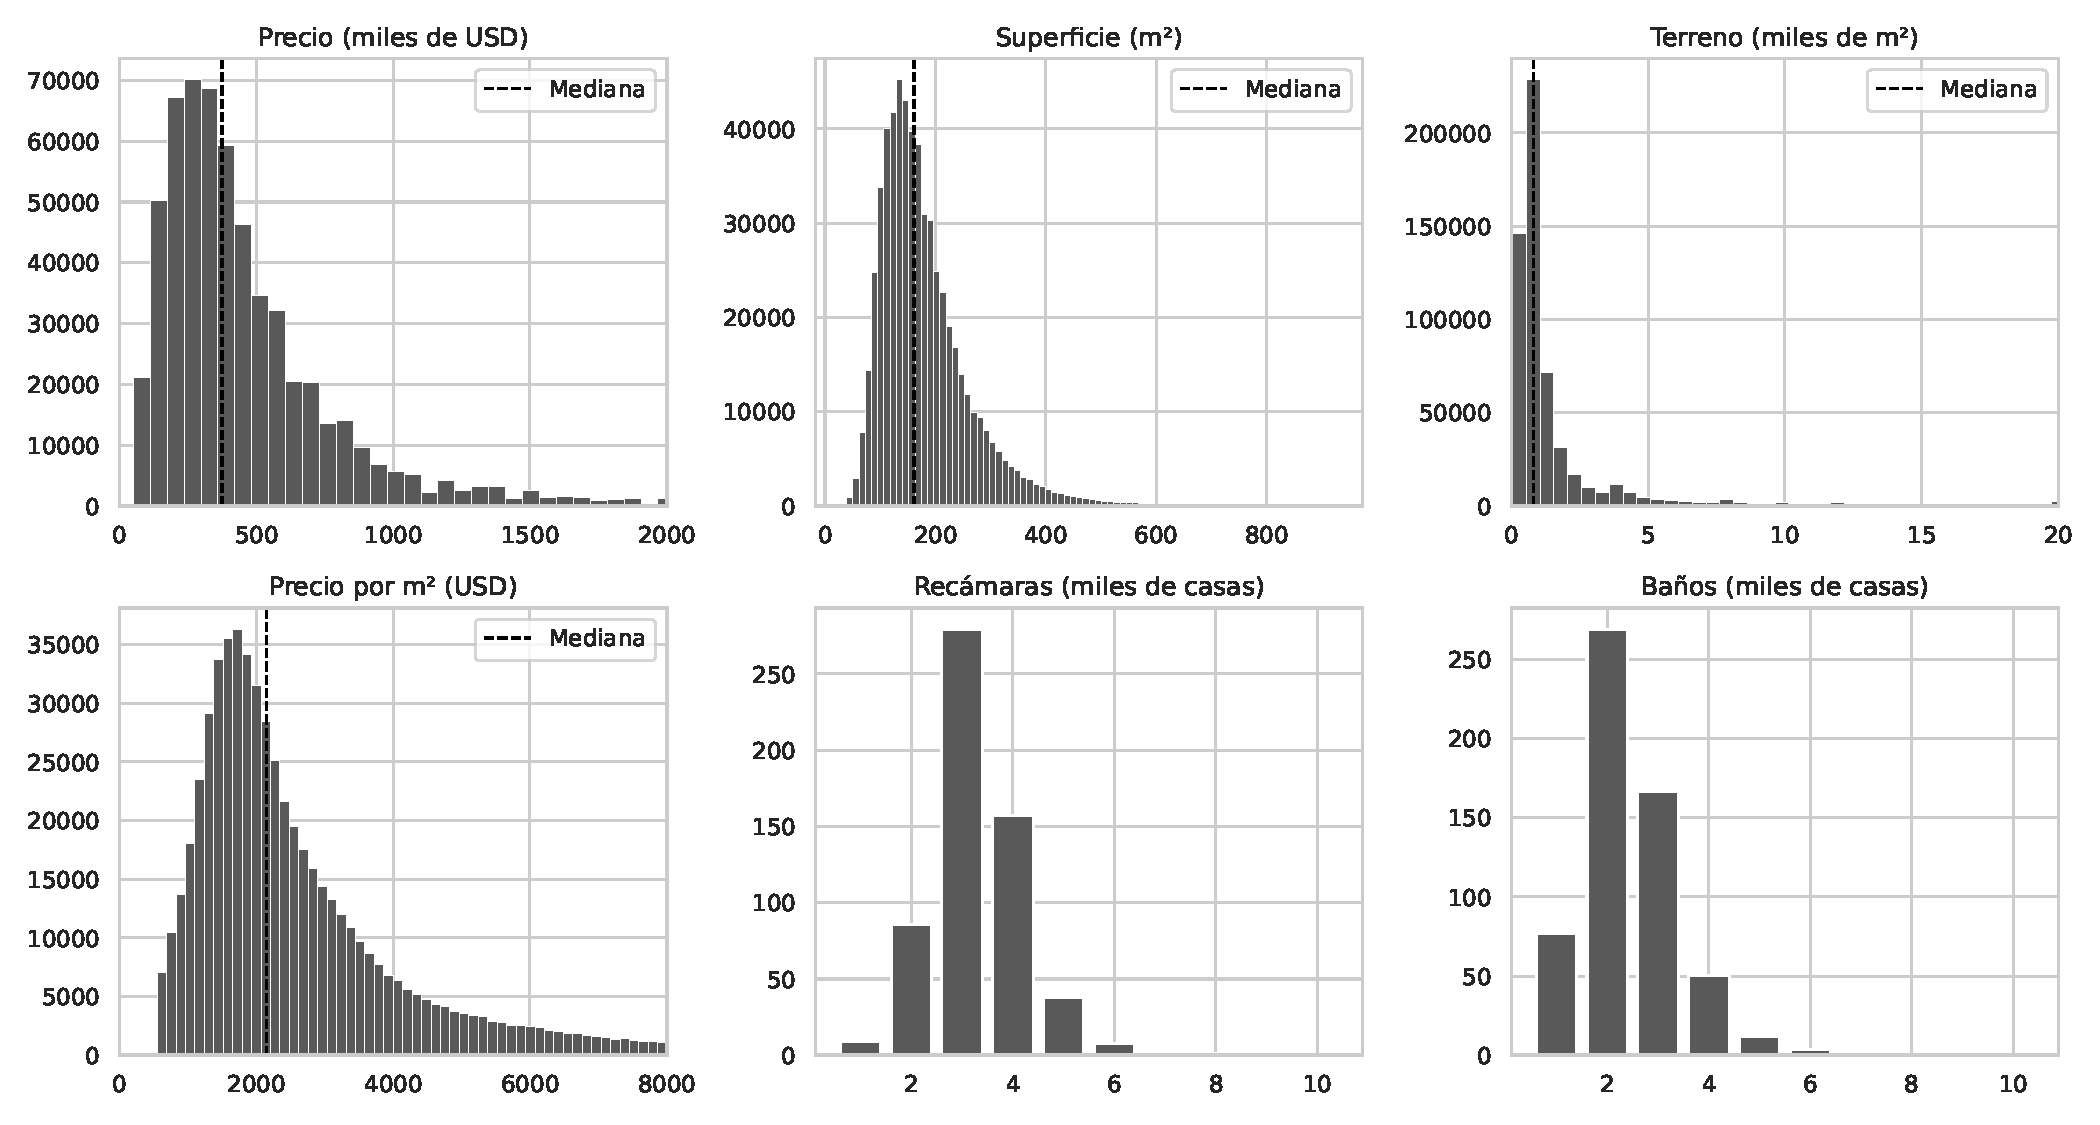
\includegraphics[width=\textwidth]{figuras/fig1_distribuciones.pdf}
\caption{Distribución de las variables principales. La línea punteada es la mediana.}
\end{figure}

\subsection{Precio por recámaras y por estado}

\begin{figure}[H]
\centering
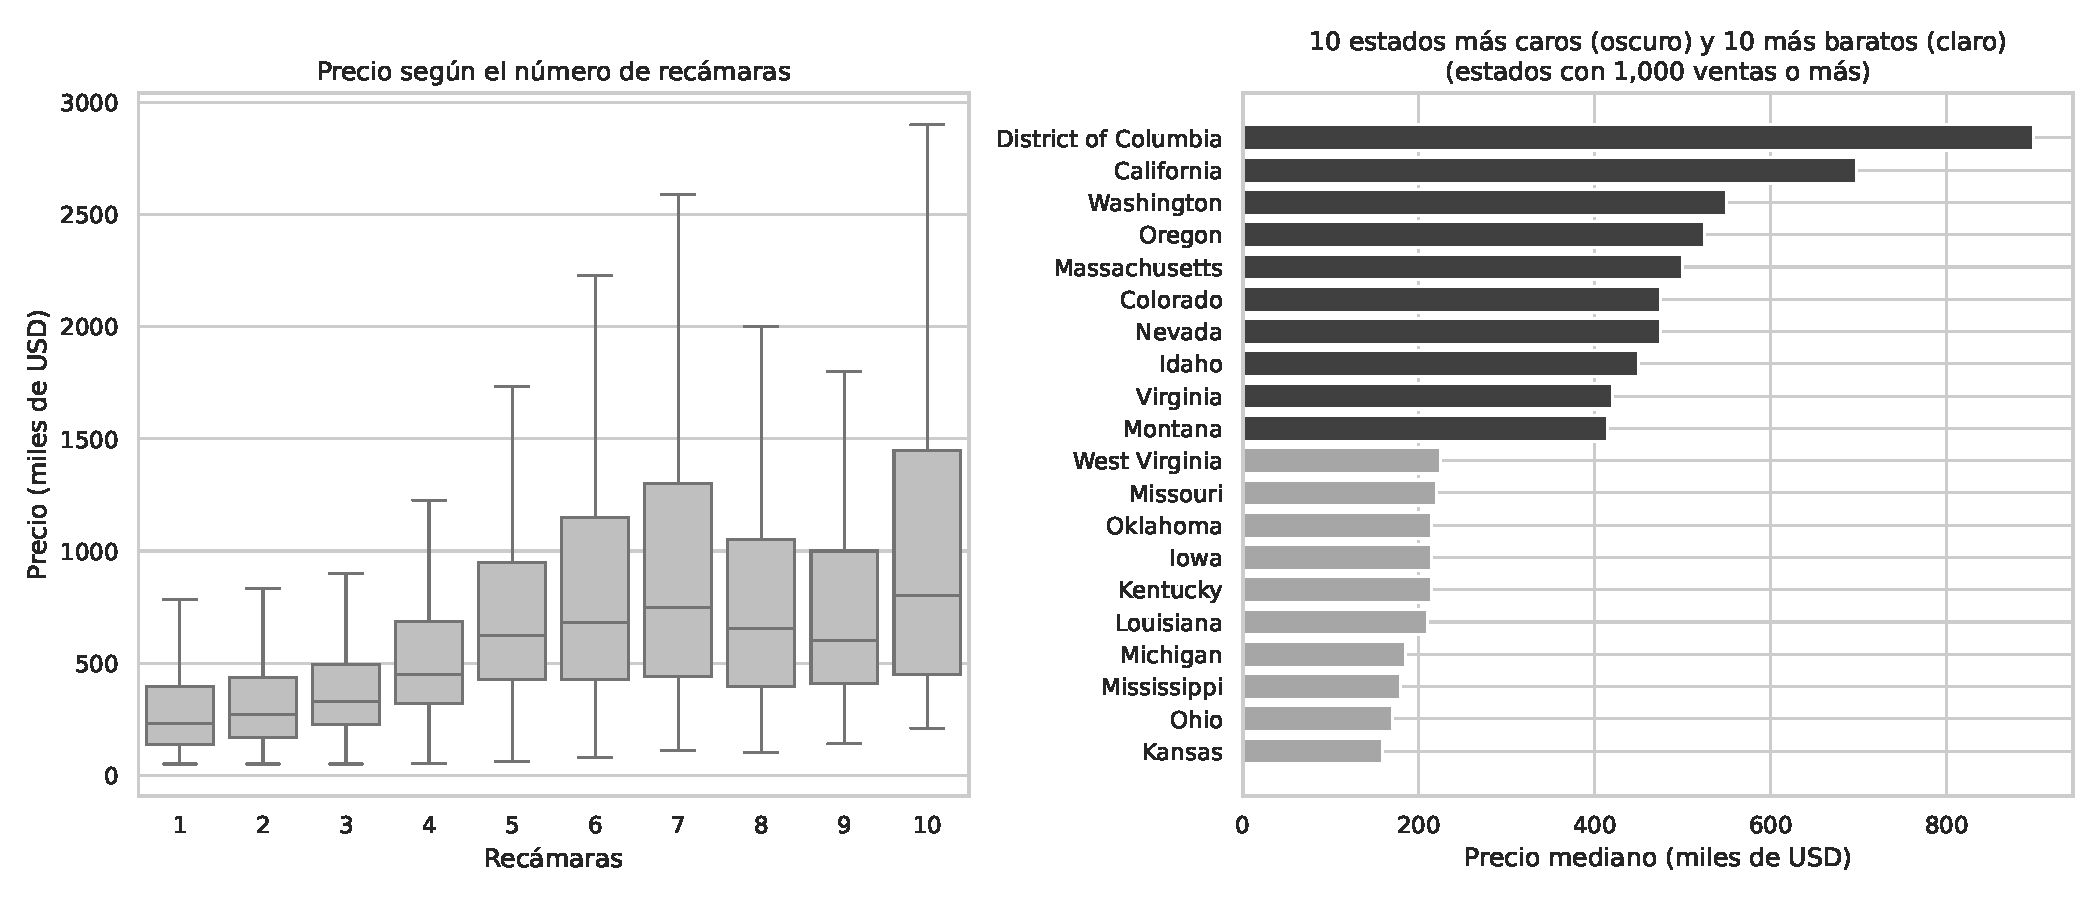
\includegraphics[width=\textwidth]{figuras/fig2_precio_recamaras_estados.pdf}
\caption{Izquierda: el precio sube con las recámaras hasta 5 o 7. Derecha: precio mediano de los estados más caros y más baratos.}
\end{figure}

Las ventas no están repartidas de forma pareja entre estados: California tiene 96,040 casas y otros estados menos de 100. Para comparar estados solo se usaron los 39 que tienen al menos 1,000 ventas (tabla~\ref{tab:estados}). La diferencia es enorme: el precio mediano de District of Columbia es 5.7 veces el de Kansas. La ubicación es, por mucho, lo que más mueve el precio.

\begin{table}[H]
\centering
\caption{Estados más caros y más baratos (con 1,000 ventas o más).}\label{tab:estados}
\small
\begin{tabular}{lrrr}
\toprule
Estado & Casas vendidas & Precio mediano (USD) & Precio mediano por m$^2$ (USD) \\
\midrule
District of Columbia & 1,653 & 899,000 & 5,049 \\
California & 96,040 & 698,000 & 4,701 \\
Washington & 29,119 & 549,999 & 3,298 \\
Oregon & 9,015 & 525,000 & 3,240 \\
Massachusetts & 21,095 & 499,900 & 3,057 \\
Louisiana & 2,038 & 210,000 & 1,302 \\
Michigan & 4,040 & 184,950 & 1,326 \\
Mississippi & 1,027 & 179,900 & 1,118 \\
Ohio & 15,399 & 169,900 & 1,143 \\
Kansas & 2,740 & 159,000 & 1,006 \\
\bottomrule
\end{tabular}
\end{table}

\subsection{Datos históricos: evolución del precio}

\begin{table}[H]
\centering
\caption{Ventas y precio mediano por mes.}
\small
\begin{tabular}{lrrr}
\toprule
Mes & Casas vendidas & Precio mediano (USD) & Precio mediano por m$^2$ (USD) \\
\midrule
2021-10 & 10,793 & 331,500 & 1,926 \\
2021-11 & 78,200 & 340,000 & 1,966 \\
2021-12 & 92,391 & 350,000 & 2,025 \\
2022-01 & 68,334 & 349,900 & 2,054 \\
2022-02 & 75,975 & 369,000 & 2,159 \\
2022-03 & 117,209 & 387,400 & 2,247 \\
2022-04 & 130,960 & 399,500 & 2,265 \\
2022-05 & 5,872 & 589,000 & 3,535 \\
\bottomrule
\end{tabular}
\end{table}

Octubre de 2021 y mayo de 2022 son meses incompletos (pocas ventas), así que no se usan para medir la tendencia. Entre 2021-11 y 2022-04 el precio mediano por m$^2$ subió \textbf{15.2\,\%} en solo cinco meses, que coincide con el alza fuerte del mercado de vivienda de Estados Unidos en ese periodo.

\begin{figure}[H]
\centering
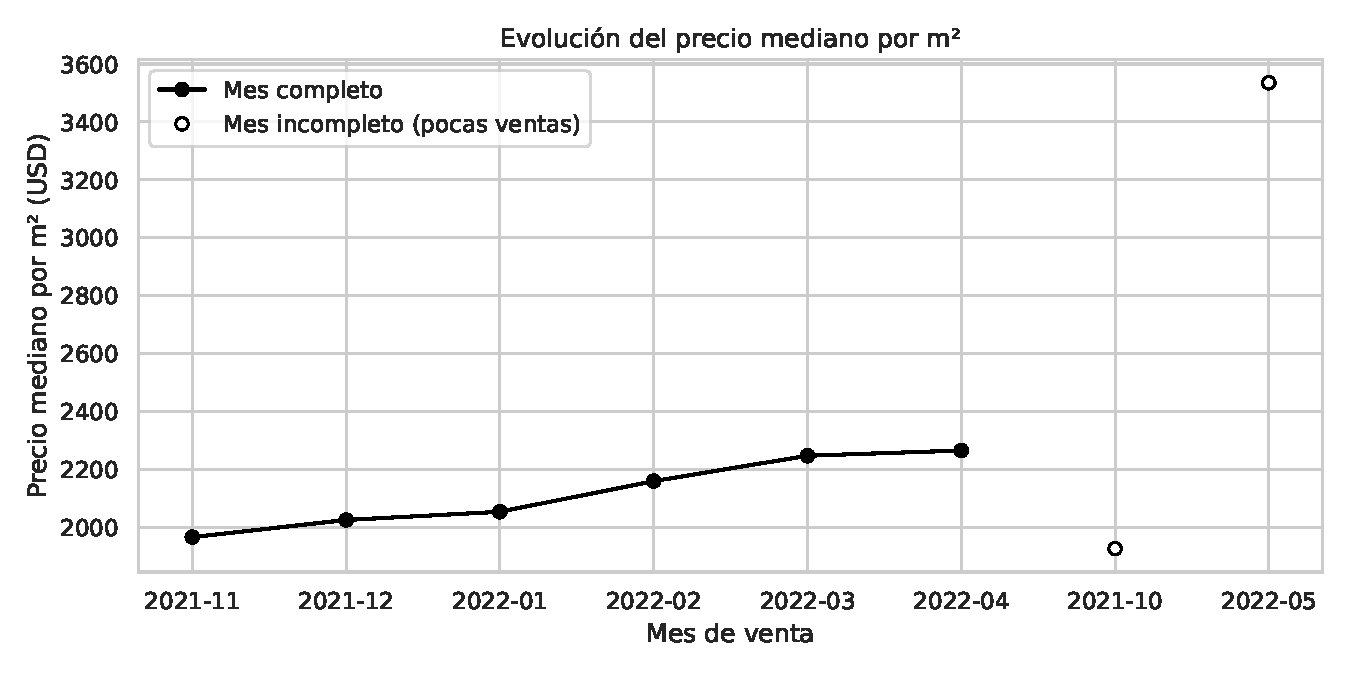
\includegraphics[width=0.7\textwidth]{figuras/fig3_precio_por_mes.pdf}
\caption{Precio mediano por m$^2$ por mes de venta.}
\end{figure}

%%%%%%%%%%%%%%%%%%%%%%%%%%%%%%%%%%%%%%%%%%%%%%%%%%%%%%%%%%%%%%%%%%%%%%%%%%%
\section{Análisis de correlación}

Se calcularon el coeficiente de Pearson (relación lineal) y el de Spearman (relación monótona con rangos, más robusto a la asimetría del precio). Se usa la escala $|r| < 0.3$ débil, $0.3 \le |r| < 0.7$ moderada y $|r| \ge 0.7$ fuerte. La significancia se prueba con
$$ t = \frac{r\sqrt{n-2}}{\sqrt{1-r^2}}, \qquad gl = n - 2, \qquad H_0: \rho = 0. $$

\begin{figure}[H]
\centering
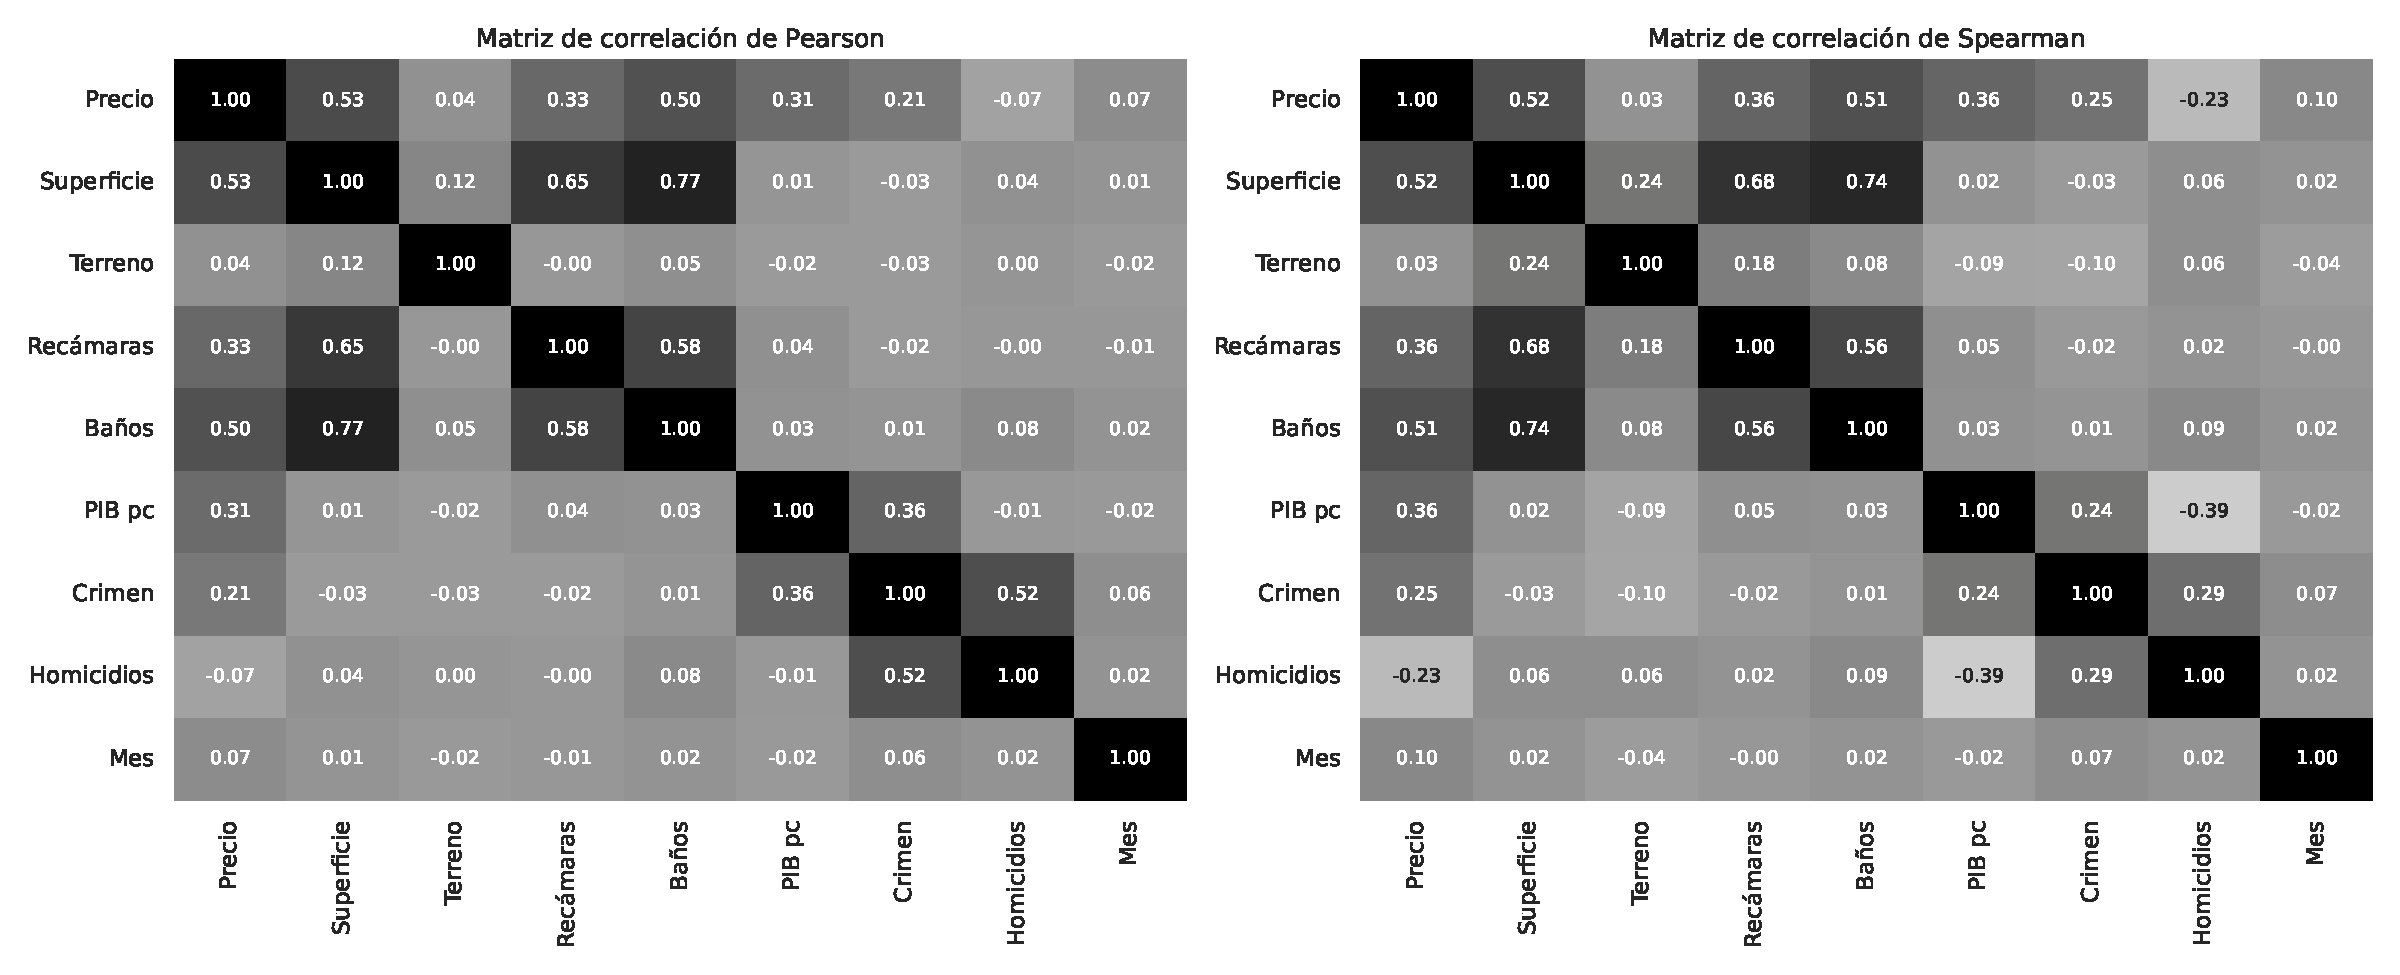
\includegraphics[width=\textwidth]{figuras/fig4_correlacion.pdf}
\caption{Matrices de correlación de Pearson y de Spearman.}
\end{figure}

\begin{table}[H]
\centering
\caption{Correlación de cada variable con el precio ($n = 579,734$).}
\small
\begin{tabular}{lrrrrl}
\toprule
Variable & $r$ Pearson & $t$ & $p$-valor & $\rho$ Spearman & Fuerza \\
\midrule
Superficie (m$^2$) & 0.5323 & 478.7 & $<0.0001$ & 0.5175 & Moderada \\
Baños & 0.5040 & 444.3 & $<0.0001$ & 0.5081 & Moderada \\
Recámaras & 0.3311 & 267.2 & $<0.0001$ & 0.3630 & Moderada \\
PIB per cápita (USD) & 0.3091 & 247.4 & $<0.0001$ & 0.3577 & Moderada \\
Crimen violento (por 100 mil) & 0.2143 & 167.0 & $<0.0001$ & 0.2547 & Débil \\
Mes de venta (0 = oct 2021) & 0.0750 & 57.2 & $<0.0001$ & 0.0976 & Débil \\
Homicidios (por 100 mil) & -0.0736 & -56.2 & $<0.0001$ & -0.2337 & Débil \\
Terreno (m$^2$) & 0.0375 & 28.6 & $<0.0001$ & 0.0295 & Débil \\
\bottomrule
\end{tabular}
\end{table}

\textbf{Interpretación.}
\begin{itemize}[nosep]
  \item La \textbf{superficie} ($r = 0.5323$) y los \textbf{baños} son los factores con mayor relación con el precio; las recámaras tienen una relación moderada pero menor, porque una casa puede tener muchas recámaras pequeñas.
  \item El \textbf{terreno} casi no se relaciona con el precio ($r = 0.0375$): los terrenos grandes suelen estar en zonas rurales, donde el suelo es barato.
  \item El \textbf{PIB per cápita} tiene una relación moderada: los estados más ricos tienen casas más caras. Con los 39 estados con 1,000 ventas o más, la correlación entre el PIB per cápita y el precio mediano por m$^2$ es $r = 0.6569$.
  \item El \textbf{crimen violento} tiene una correlación positiva débil con el precio. No significa que el crimen suba el precio: los estados con más crimen por habitante (como California o Washington D.C.) también son urbanos y caros. Es una correlación \textbf{espuria} explicada por una tercera variable. En la regresión, al controlar la zona, el signo se vuelve negativo (sección~\ref{sec:regresion}).
  \item Con más de medio millón de casas \textbf{todas} las correlaciones son significativas ($p < 0.05$), incluso las muy pequeñas. Por eso se interpreta sobre todo el tamaño de $r$.
\end{itemize}

\begin{figure}[H]
\centering
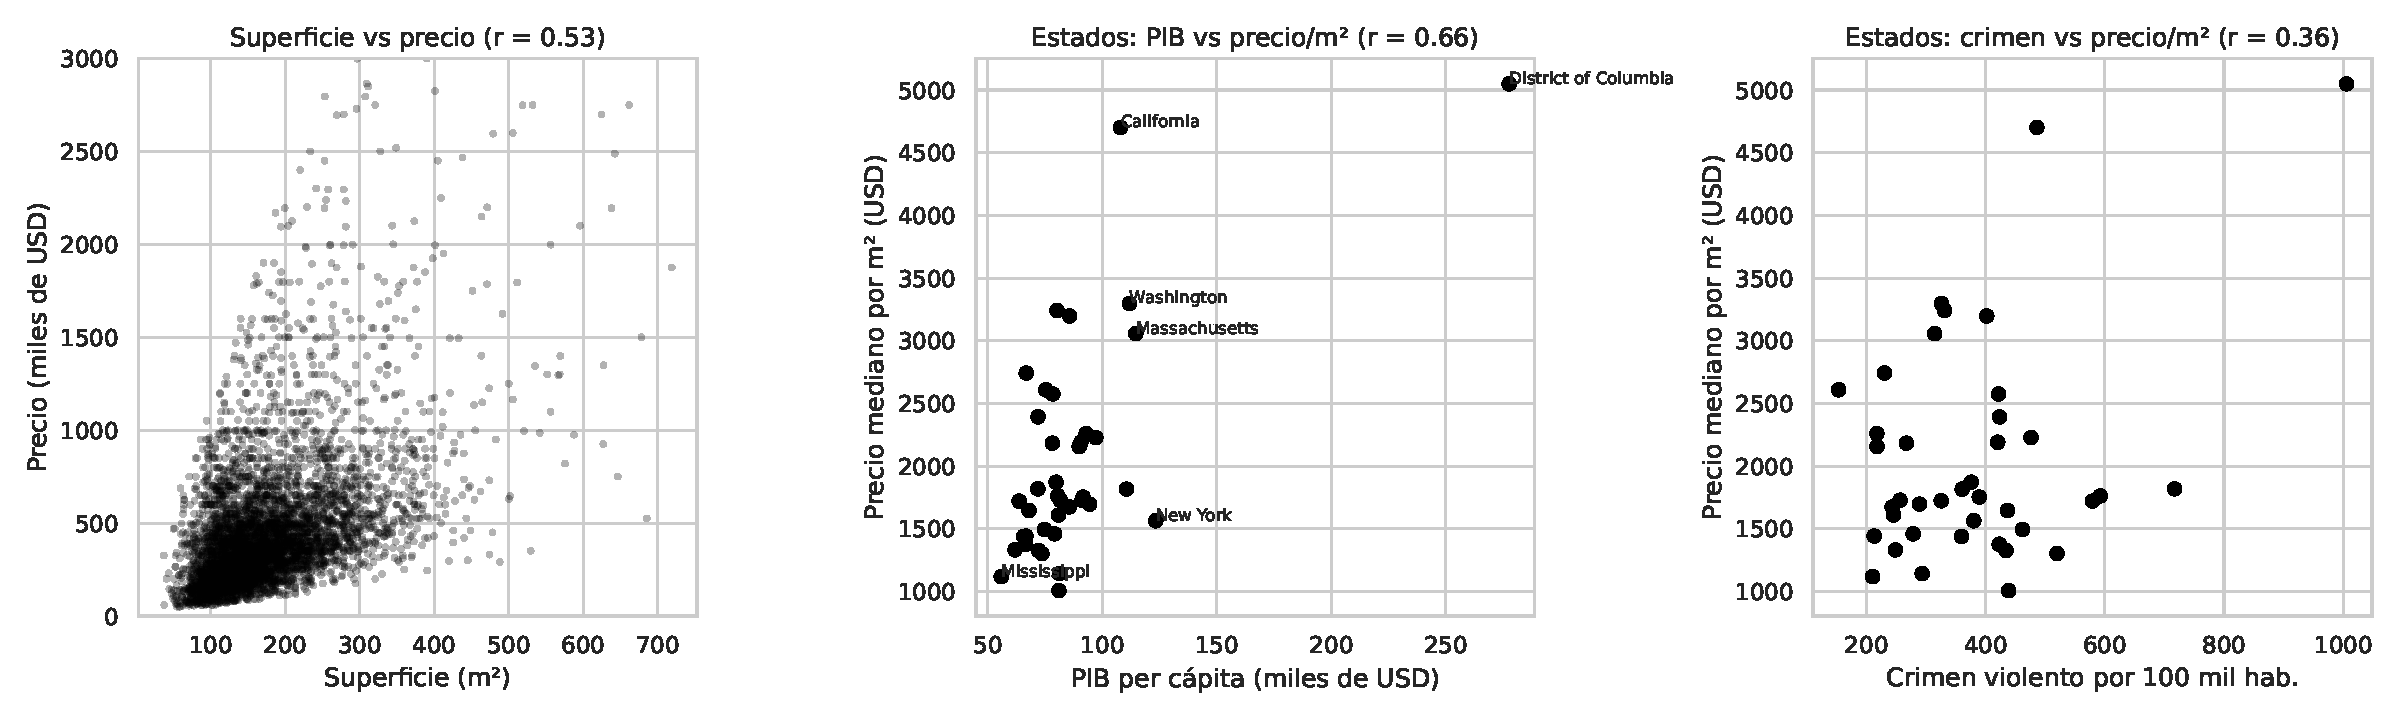
\includegraphics[width=\textwidth]{figuras/fig5_dispersion.pdf}
\caption{Superficie contra precio (5,000 casas al azar) y relación por estado del PIB per cápita y del crimen con el precio por m$^2$.}
\end{figure}

%%%%%%%%%%%%%%%%%%%%%%%%%%%%%%%%%%%%%%%%%%%%%%%%%%%%%%%%%%%%%%%%%%%%%%%%%%%
\section{Modelado estadístico: regresión lineal múltiple}\label{sec:regresion}

Los coeficientes se calcularon por \textbf{mínimos cuadrados con matrices},
$$ \mathbf{b} = \paren{\mathbf{X}'\mathbf{X}}^{-1}\mathbf{X}'\mathbf{y}, $$
donde la primera columna de $\mathbf{X}$ es de unos. El desarrollo con las matrices está en el Anexo~\ref{sec:anexo}. Los resultados se comprobaron con statsmodels.

\subsection{Modelo 1: características de la casa e indicadores del estado}

$$ \hat{y} = b_0 + b_1\,\text{Sup} + b_2\,\text{Terr} + b_3\,\text{Rec} + b_4\,\text{Baños} + b_5\,\text{PIB} + b_6\,\text{Crimen} + b_7\,\text{Mes} $$

\begin{table}[H]
\centering
\caption{Modelo 1: coeficientes ($R^2 = 0.4171$ en entrenamiento, $F = 47,400$).}
\small
\begin{tabular}{lrrrr}
\toprule
Variable & Coeficiente & Error est. & $t$ & $p$-valor \\
\midrule
Intercepto & -778110.2159 & 3130.5535 & -248.55 & $<0.0001$ \\
Superficie (m$^2$) & 1991.3590 & 9.2664 & 214.90 & $<0.0001$ \\
Terreno (m$^2$) & -1.0298 & 0.1055 & -9.76 & $<0.0001$ \\
Recámaras & -29908.5427 & 645.1280 & -46.36 & $<0.0001$ \\
Baños & 90715.5957 & 741.3966 & 122.36 & $<0.0001$ \\
PIB per cápita (USD) & 5.9369 & 0.0276 & 215.19 & $<0.0001$ \\
Crimen violento (por 100 mil) & 494.3477 & 4.7875 & 103.26 & $<0.0001$ \\
Mes de venta & 14351.3502 & 249.9414 & 57.42 & $<0.0001$ \\
\bottomrule
\end{tabular}
\end{table}

El modelo 1 explica solo el 42\,\% de la variación del precio. Las características de la casa y los indicadores del estado no bastan, porque dentro de un mismo estado hay zonas muy baratas y muy caras. Además, el crimen sale con coeficiente positivo (494.3 USD por punto), que es la correlación espuria descrita arriba.

\subsection{Modelo 2: se agrega el precio por m$^2$ de la zona}

Para medir la ubicación fina se agregó el \textbf{precio mediano por m$^2$ del código postal}, calculado solo con las ventas del conjunto de entrenamiento. Es el dato histórico de precios de la zona.

\begin{table}[H]
\centering
\caption{Modelo 2: coeficientes ($R^2 = 0.7531$, $R^2_{aj} = 0.7531$, $F = 176,791$).}
\small
\begin{tabular}{lrrrr}
\toprule
Variable & Coeficiente & Error est. & $t$ & $p$-valor \\
\midrule
Intercepto & -481280.8266 & 2071.5078 & -232.33 & $<0.0001$ \\
Superficie (m$^2$) & 2215.9234 & 6.0377 & 367.01 & $<0.0001$ \\
Terreno (m$^2$) & 0.8347 & 0.0687 & 12.15 & $<0.0001$ \\
Recámaras & -6302.9994 & 420.9334 & -14.97 & $<0.0001$ \\
Baños & 42792.2709 & 486.2964 & 88.00 & $<0.0001$ \\
PIB per cápita (USD) & 0.1480 & 0.0194 & 7.64 & $<0.0001$ \\
Crimen violento (por 100 mil) & -39.5694 & 3.1876 & -12.41 & $<0.0001$ \\
Mes de venta  & 6504.6741 & 162.9746 & 39.91 & $<0.0001$ \\
Precio por m$^2$ de la zona (USD) & 170.2703 & 0.2143 & 794.39 & $<0.0001$ \\
\bottomrule
\end{tabular}
\end{table}

\textbf{Interpretación de los coeficientes} (cada uno con las demás variables constantes):
\begin{itemize}[nosep]
  \item Cada m$^2$ de construcción suma 2,216 USD, y cada baño 42,792 USD.
  \item Una recámara más \textbf{resta} 6,303 USD: con la misma superficie, más recámaras significan cuartos más chicos.
  \item El terreno aporta poco (0.83 USD por m$^2$).
  \item 1,000 USD más de PIB per cápita en el estado suben el precio 148 USD.
  \item Con la zona controlada, el crimen ya es \textbf{negativo}: 100 delitos violentos más por cada 100 mil habitantes bajan el precio 3,957 USD.
  \item Cada mes que pasa el precio sube 6,505 USD (tendencia del mercado).
  \item Si el m$^2$ de la zona cuesta 1,000 USD más, la casa vale 170,270 USD más. Es la variable con el estadístico $t$ más grande.
\end{itemize}

Todas las variables son significativas ($p < 0.05$). Los factores de inflación de la varianza son bajos (tabla~\ref{tab:vif}), así que no hay multicolinealidad grave.

\begin{table}[H]
\centering
\caption{Factor de inflación de la varianza (VIF) del modelo 2.}\label{tab:vif}
\small
\begin{tabular}{lr}
\toprule
Variable & VIF \\
\midrule
Superficie (m$^2$) & 2.94 \\
Terreno (m$^2$) & 1.03 \\
Recámaras & 1.80 \\
Baños & 2.54 \\
PIB per cápita (USD) & 1.35 \\
Crimen violento (por 100 mil) & 1.21 \\
Mes de venta  & 1.01 \\
Precio por m$^2$ de la zona (USD) & 1.35 \\
\bottomrule
\end{tabular}
\end{table}

\subsection{Métricas de la regresión en el conjunto de prueba}

\begin{table}[H]
\centering
\caption{Métricas de los modelos lineales (conjunto de prueba).}
\small
\begin{tabular}{lrrrr}
\toprule
Modelo & MSE (USD$^2$) & RMSE (USD) & MAE (USD) & $R^2$ \\
\midrule
Regresión lineal 1 (sin zona) & $9.6943\times10^{10}$ & 311,356 & 195,172 & 0.4192 \\
Regresión lineal 2 (con zona) & $4.1729\times10^{10}$ & 204,276 & 116,808 & 0.7500 \\
\bottomrule
\end{tabular}
\end{table}

Al agregar la zona, el $R^2$ sube de 0.42 a 0.75 y el error medio absoluto baja de 195,172 a 116,808 USD. Las métricas de prueba son casi iguales a las de entrenamiento, así que el modelo no está sobreajustado.

Una limitación de la regresión lineal es que \textbf{suma} los efectos: 1 m$^2$ extra vale lo mismo en Mississippi que en Manhattan. En realidad el valor de un m$^2$ depende de la zona (es una interacción), y eso es lo que pueden captar los modelos de \emph{machine learning}.

%%%%%%%%%%%%%%%%%%%%%%%%%%%%%%%%%%%%%%%%%%%%%%%%%%%%%%%%%%%%%%%%%%%%%%%%%%%
\section{Modelado predictivo con machine learning}

Se entrenaron cinco modelos con las mismas 8 variables del modelo lineal 2 y los mismos conjuntos de entrenamiento y prueba.

\begin{table}[H]
\centering
\caption{Modelos de \emph{machine learning} y su configuración.}
\small
\begin{tabular}{p{3.6cm}p{11.2cm}}
\toprule
Modelo & Idea y configuración \\
\midrule
K vecinos (KNN) & Promedia el precio de las $k = 10$ casas más parecidas. Variables estandarizadas ($z = (x - \bar{x})/s$). \\
Árbol de decisión & Divide las casas con reglas del tipo ``si la superficie es mayor que 150 m$^2$\dots''. Profundidad máxima 12, mínimo 20 casas por hoja. \\
Random Forest & Promedio de 100 árboles, cada uno entrenado con una muestra distinta. Profundidad máxima 20, mínimo 5 casas por hoja. \\
XGBoost & \emph{Gradient boosting}: 500 árboles pequeños (profundidad 8), cada uno corrige los errores de los anteriores. Tasa de aprendizaje 0.05. \\
Red neuronal (MLP) & Perceptrón multicapa con dos capas ocultas de 64 y 32 neuronas, optimizador Adam y paro temprano. Variables estandarizadas. \\
\bottomrule
\end{tabular}
\end{table}

%%%%%%%%%%%%%%%%%%%%%%%%%%%%%%%%%%%%%%%%%%%%%%%%%%%%%%%%%%%%%%%%%%%%%%%%%%%
\section{Evaluación y comparación de modelos}\label{sec:comparacion}

Métricas usadas, con $y_i$ el precio real, $\hat{y}_i$ el predicho y $n$ el número de casas de prueba:
$$ MSE = \frac{1}{n}\sum \paren{y_i - \hat{y}_i}^2 \qquad RMSE = \sqrt{MSE} $$
$$ MAE = \frac{1}{n}\sum \left|y_i - \hat{y}_i\right| \qquad R^2 = 1 - \frac{\sum \paren{y_i - \hat{y}_i}^2}{\sum \paren{y_i - \bar{y}}^2} $$

\begin{table}[H]
\centering
\caption{Comparación de los modelos en el conjunto de prueba (115,947 casas), ordenados por $R^2$.}
\footnotesize\setlength{\tabcolsep}{4pt}
\begin{tabular}{lrrrrr}
\toprule
Modelo & MSE (USD$^2$) & RMSE (USD) & MAE (USD) & $R^2$ & Tiempo (s) \\
\midrule
XGBoost & $2.1239\times10^{10}$ & 145,737 & 78,284 & 0.8727 & 6.4 \\
Random Forest & $2.1811\times10^{10}$ & 147,686 & 78,220 & 0.8693 & 37.2 \\
Red neuronal (MLP) & $2.5148\times10^{10}$ & 158,581 & 86,691 & 0.8493 & 135.6 \\
Árbol de decisión & $2.5531\times10^{10}$ & 159,784 & 85,531 & 0.8470 & 1.6 \\
KNN (k = 10) & $2.5877\times10^{10}$ & 160,863 & 86,531 & 0.8450 & 10.3 \\
Regresión lineal 2 (con zona) & $4.1729\times10^{10}$ & 204,276 & 116,808 & 0.7500 & -- \\
Regresión lineal 1 (sin zona) & $9.6943\times10^{10}$ & 311,356 & 195,172 & 0.4192 & -- \\
\bottomrule
\end{tabular}
\end{table}

\begin{figure}[H]
\centering
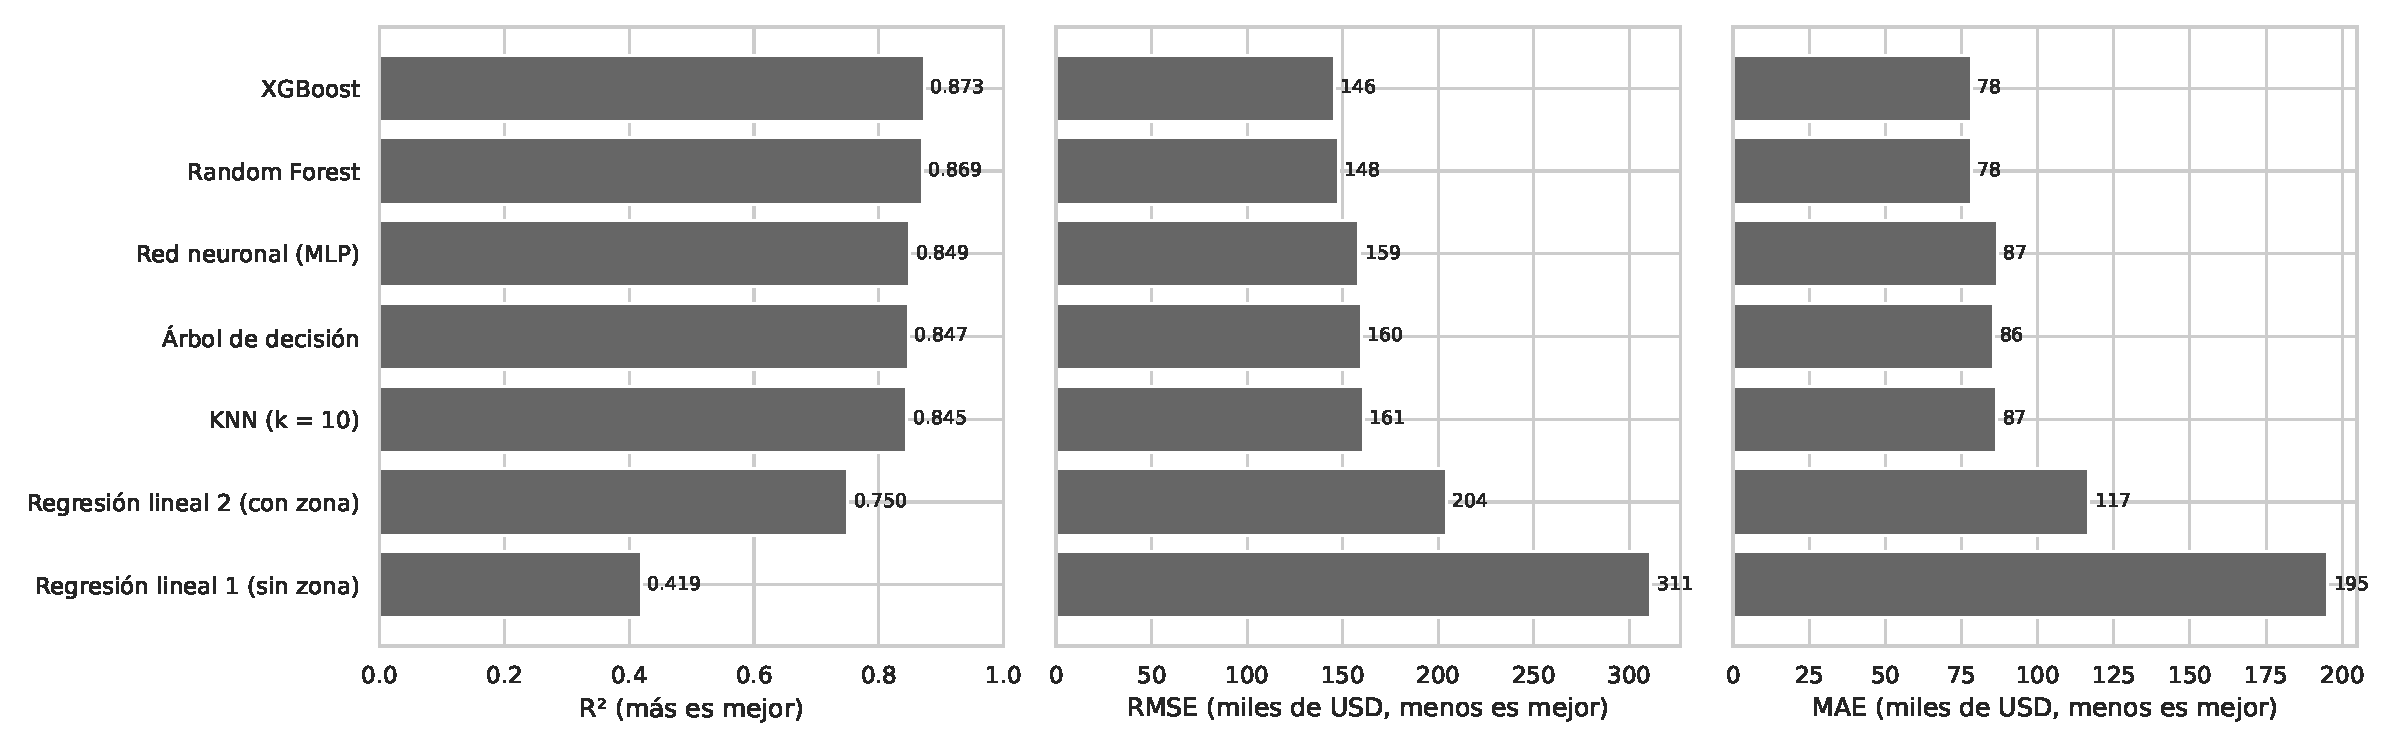
\includegraphics[width=\textwidth]{figuras/fig6_comparacion_modelos.pdf}
\caption{Comparación de $R^2$, RMSE y MAE.}
\end{figure}

\textbf{Resultados.}
\begin{itemize}[nosep]
  \item \textbf{XGBoost} es el mejor modelo: explica el 87.3\,\% de la variación del precio, con RMSE de 145,737 USD y MAE de 78,284 USD. Además es de los más rápidos (6 s).
  \item \textbf{Random Forest} queda prácticamente empatado (MAE de 78,220 USD, incluso un poco menor, y $R^2 = 0.8693$), pero tarda 6 veces más y el modelo guardado ocupa mucho más espacio.
  \item La red neuronal, el árbol de decisión y KNN quedan cerca entre sí ($R^2 \approx 0.85$).
  \item Todos los modelos de \emph{machine learning} superan a la regresión lineal 2: XGBoost reduce el MAE en 33\,\%. El error porcentual mediano baja de 19.9\,\% con la regresión lineal a 12.2\,\% con XGBoost.
\end{itemize}

\begin{figure}[H]
\centering
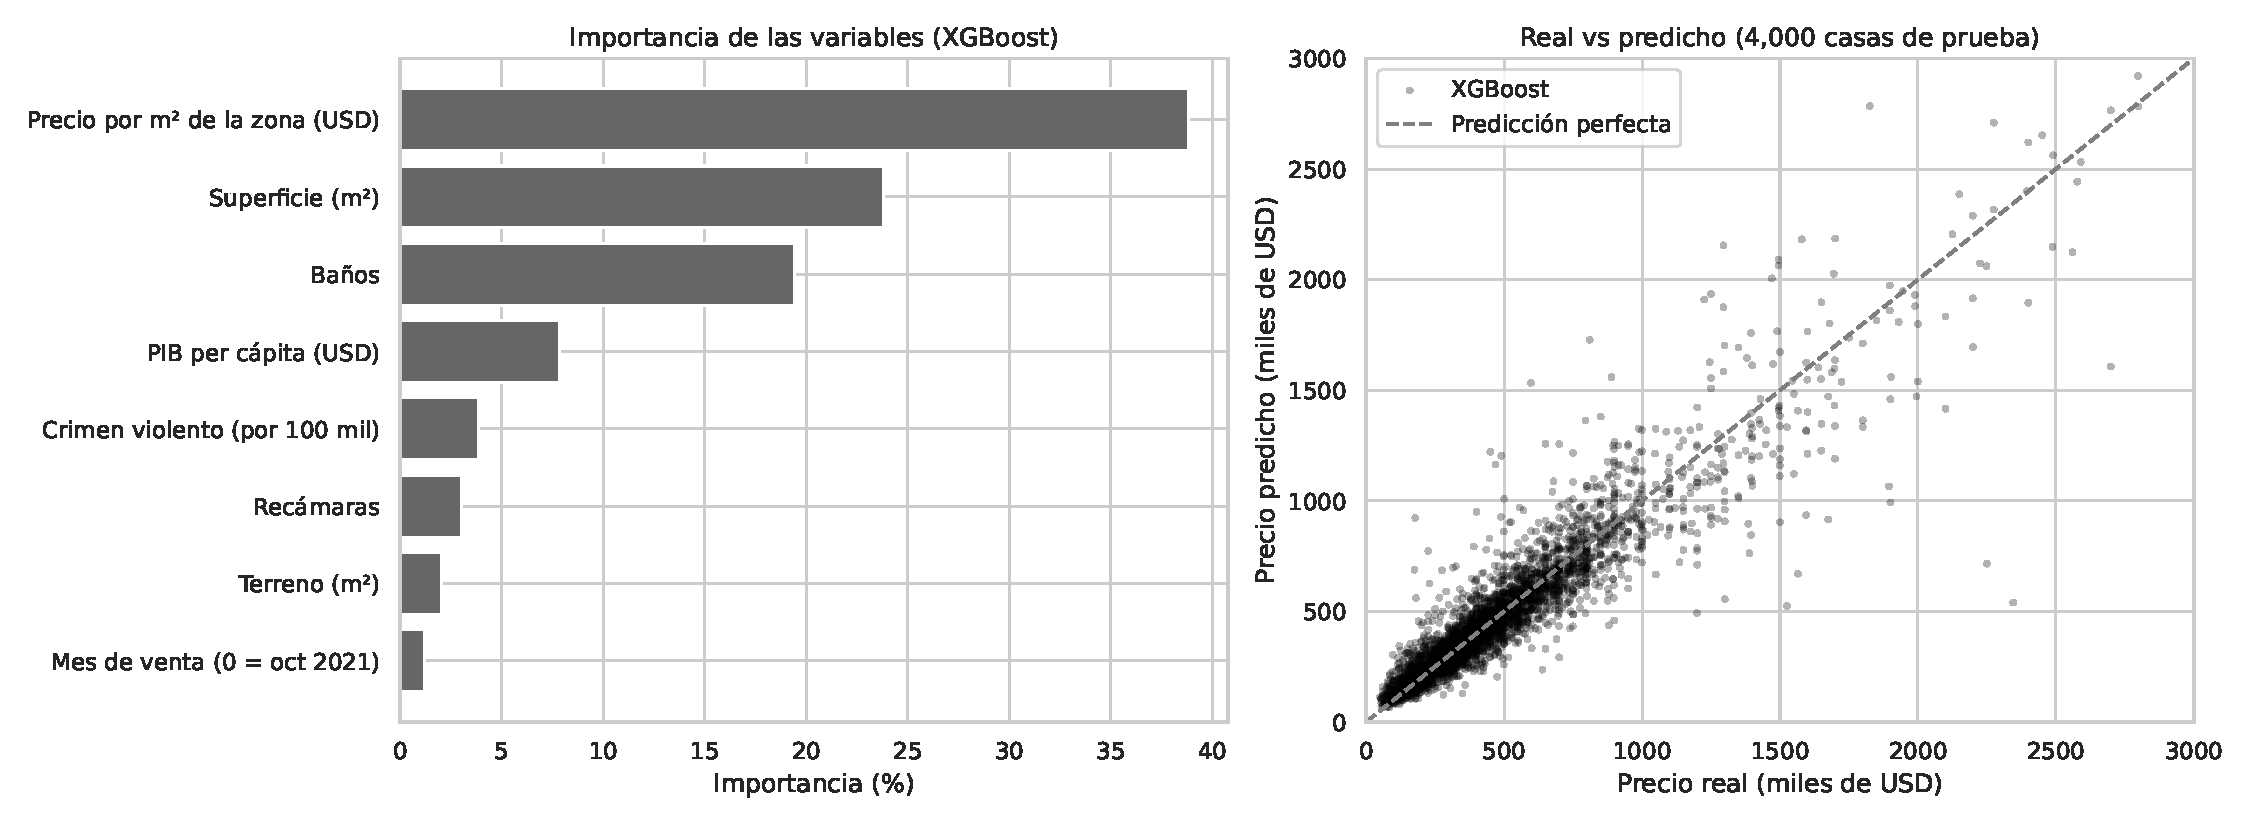
\includegraphics[width=\textwidth]{figuras/fig7_importancia_real_vs_predicho.pdf}
\caption{Importancia de las variables en XGBoost y precio real contra predicho.}
\end{figure}

\begin{table}[H]
\centering
\caption{Importancia de las variables en XGBoost.}
\small
\begin{tabular}{lr}
\toprule
Variable & Importancia (\%) \\
\midrule
Precio por m$^2$ de la zona (USD) & 38.8 \\
Superficie (m$^2$) & 23.8 \\
Baños & 19.4 \\
PIB per cápita (USD) & 7.8 \\
Crimen violento (por 100 mil) & 3.8 \\
Recámaras & 3.0 \\
Terreno (m$^2$) & 2.0 \\
Mes de venta  & 1.2 \\
\bottomrule
\end{tabular}
\end{table}

La importancia confirma lo que mostró la correlación: la zona, la superficie y los baños son lo que más pesa. Los indicadores del estado aportan menos porque el precio de la zona ya contiene buena parte de esa información.

\begin{figure}[H]
\centering
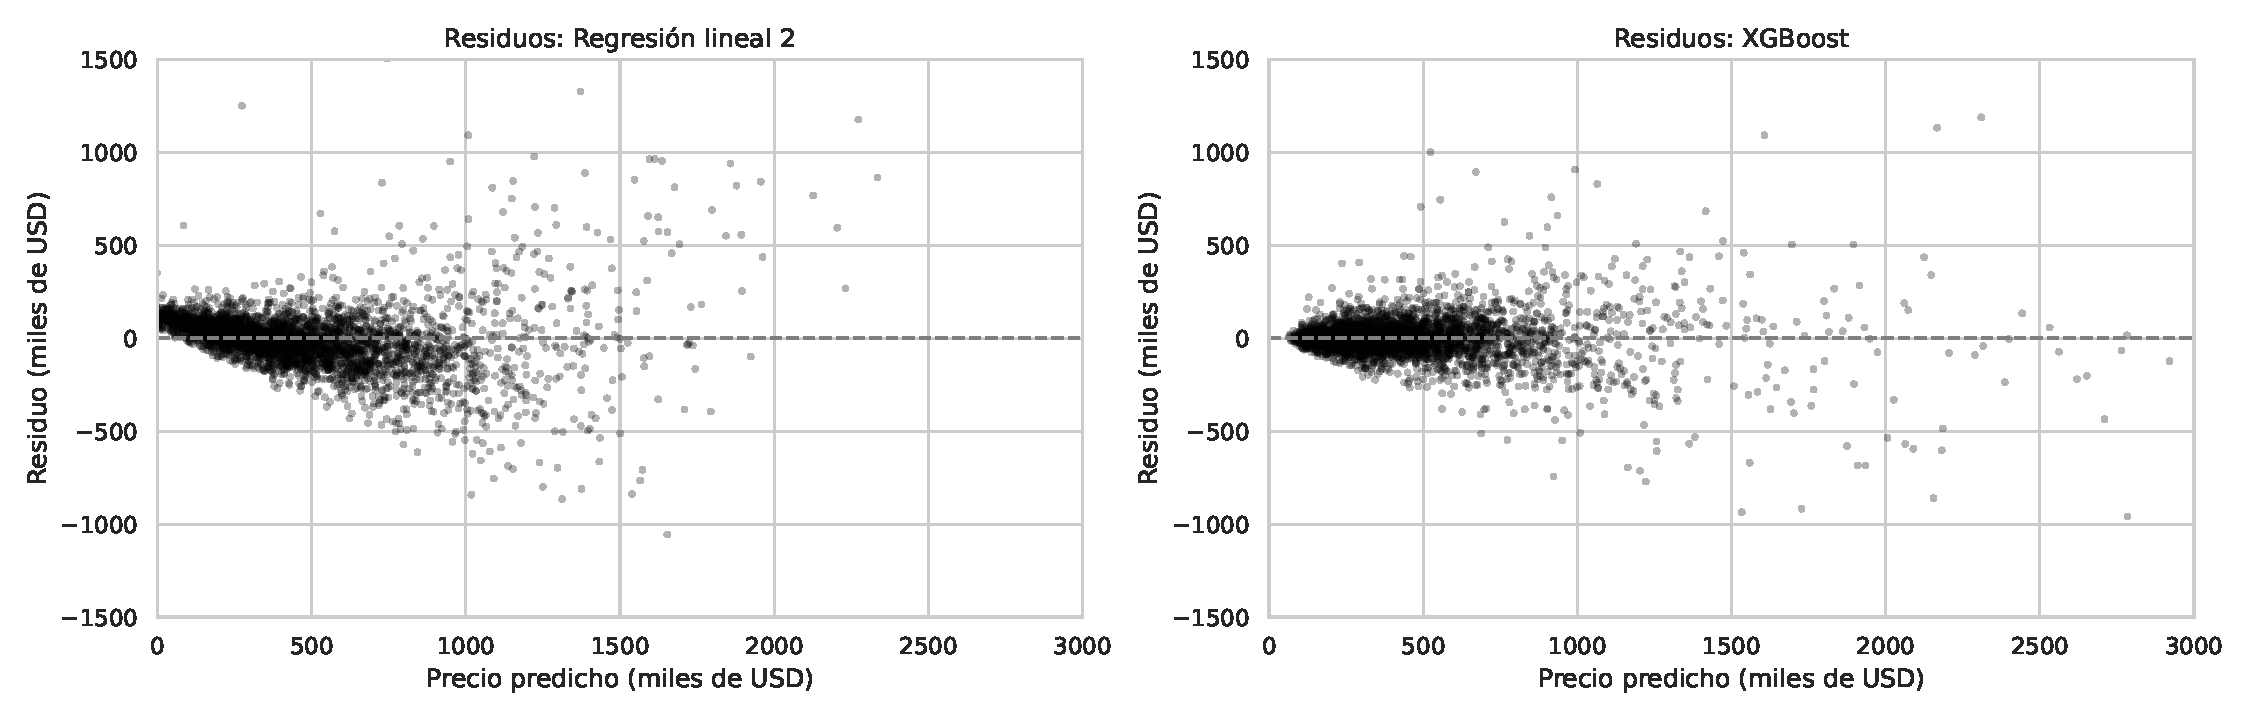
\includegraphics[width=\textwidth]{figuras/fig8_residuos.pdf}
\caption{Residuos de la regresión lineal 2 y de XGBoost. Los de XGBoost están más concentrados alrededor de cero.}
\end{figure}

\begin{table}[H]
\centering
\caption{Error de XGBoost por rango de precio real.}
\small
\begin{tabular}{lrrr}
\toprule
Rango de precio (USD) & Casas & MAE (USD) & Error porcentual mediano (\%) \\
\midrule
< 200 mil & 20,842 & 43,997 & 20.2 \\
200 a 400 mil & 44,189 & 47,043 & 11.4 \\
400 a 800 mil & 37,100 & 78,471 & 10.5 \\
> 800 mil & 13,816 & 229,421 & 12.8 \\
\bottomrule
\end{tabular}
\end{table}

En pesos absolutos el error crece con el precio (es más difícil acertar en casas de lujo), pero en porcentaje el modelo funciona mejor entre 200 mil y 800 mil USD, donde está la mayoría de las casas. Las casas de menos de 200 mil USD tienen el mayor error porcentual.

\subsection{Ejemplo de predicción}

Casa de 180 m$^2$ de construcción, terreno de 600 m$^2$, 3 recámaras y 2 baños, vendida en mayo de 2022 en el código postal 78745 (Austin, Texas), donde el m$^2$ cuesta 1,753 USD:
\begin{itemize}[nosep]
  \item Regresión lineal 2: \textbf{326,896 USD}.
  \item XGBoost: \textbf{324,496 USD}.
\end{itemize}
En el dashboard se puede hacer esta estimación para cualquier estado, ciudad y código postal del dataset.

%%%%%%%%%%%%%%%%%%%%%%%%%%%%%%%%%%%%%%%%%%%%%%%%%%%%%%%%%%%%%%%%%%%%%%%%%%%
\section{Hallazgos y recomendaciones}

\begin{enumerate}[nosep]
  \item \textbf{La ubicación manda.} El precio histórico por m$^2$ de la zona es la variable más importante en todos los modelos. Para valuar una casa, lo primero es conocer las ventas recientes de su código postal.
  \item \textbf{Superficie y baños} son las características de la casa que más suben el precio. Más recámaras sin más superficie no suben el valor.
  \item \textbf{El entorno económico importa}, pero a nivel de estado es poco preciso: el PIB per cápita sube el precio y el crimen lo baja una vez que se controla la zona.
  \item \textbf{El mercado subió rápido:} 15.2\,\% en el precio por m$^2$ en cinco meses. Un modelo de precios debe actualizarse con ventas recientes.
  \item \textbf{Modelo recomendado: XGBoost}, por tener el mejor $R^2$, un MAE casi igual al menor y un tiempo de entrenamiento corto. La regresión lineal 2 se recomienda como modelo \emph{explicativo}, porque sus coeficientes se interpretan directamente.
\end{enumerate}

\section{Limitaciones}\label{sec:limitaciones}

\begin{itemize}[nosep]
  \item El dataset no incluye acceso a servicios (escuelas, transporte, hospitales) ni coordenadas, que el caso menciona. Se podrían agregar con datos del censo por código postal.
  \item Los indicadores económicos son por estado y de años posteriores a las ventas (PIB 2025, crimen 2024); todas las casas de un estado comparten el mismo valor.
  \item Las ventas abarcan solo siete meses y algunos estados tienen muy pocas casas; Alaska y Maine quedaron sin datos.
  \item El dataset no trae características de calidad (año de construcción, estado de conservación, alberca, etc.), que explican parte del error restante.
\end{itemize}

%%%%%%%%%%%%%%%%%%%%%%%%%%%%%%%%%%%%%%%%%%%%%%%%%%%%%%%%%%%%%%%%%%%%%%%%%%%
\section{Conclusiones}

Con 579,734 casas vendidas en Estados Unidos se identificó que la superficie, los baños y, sobre todo, la ubicación son los factores que más influyen en el precio. La regresión lineal múltiple, calculada por matrices, explica el 75\,\% de la variación cuando incluye el precio de la zona, y permite interpretar cada factor. Los modelos de \emph{machine learning} mejoran la precisión porque captan que el valor de un m$^2$ depende de dónde está la casa: XGBoost alcanzó $R^2 = 0.8727$ y un error medio de 78,284 USD, por lo que es el modelo seleccionado para la implementación.

%%%%%%%%%%%%%%%%%%%%%%%%%%%%%%%%%%%%%%%%%%%%%%%%%%%%%%%%%%%%%%%%%%%%%%%%%%%
\section{Entregables}

{\raggedright
\begin{enumerate}[nosep]
  \item \textbf{Dataset:} carpeta \texttt{dataset/}, con \texttt{datos\_propiedades\_limpios.csv.gz} (dataset limpio con los indicadores, comprimido) e \texttt{indicadores\_estados.csv}. El archivo original \texttt{realtor-data.zip.csv} se descarga de Kaggle.
  \item \textbf{Informe técnico:} este documento, en la carpeta \texttt{reporte/}.
  \item \textbf{Modelos con métricas:} carpeta \texttt{modelos/}, con \texttt{metricas\_modelos.csv}, \texttt{modelo\_xgboost.json} y \texttt{coeficientes\_regresion.csv}.
  \item \textbf{Código:} \texttt{Proyecto\_final\_2\_analisis.ipynb} (Python).
  \item \textbf{Dashboard:} \texttt{app\_dashboard.py} (Streamlit), se ejecuta con \texttt{streamlit run app\_dashboard.py}.
\end{enumerate}
\par}

\begin{figure}[H]
\centering
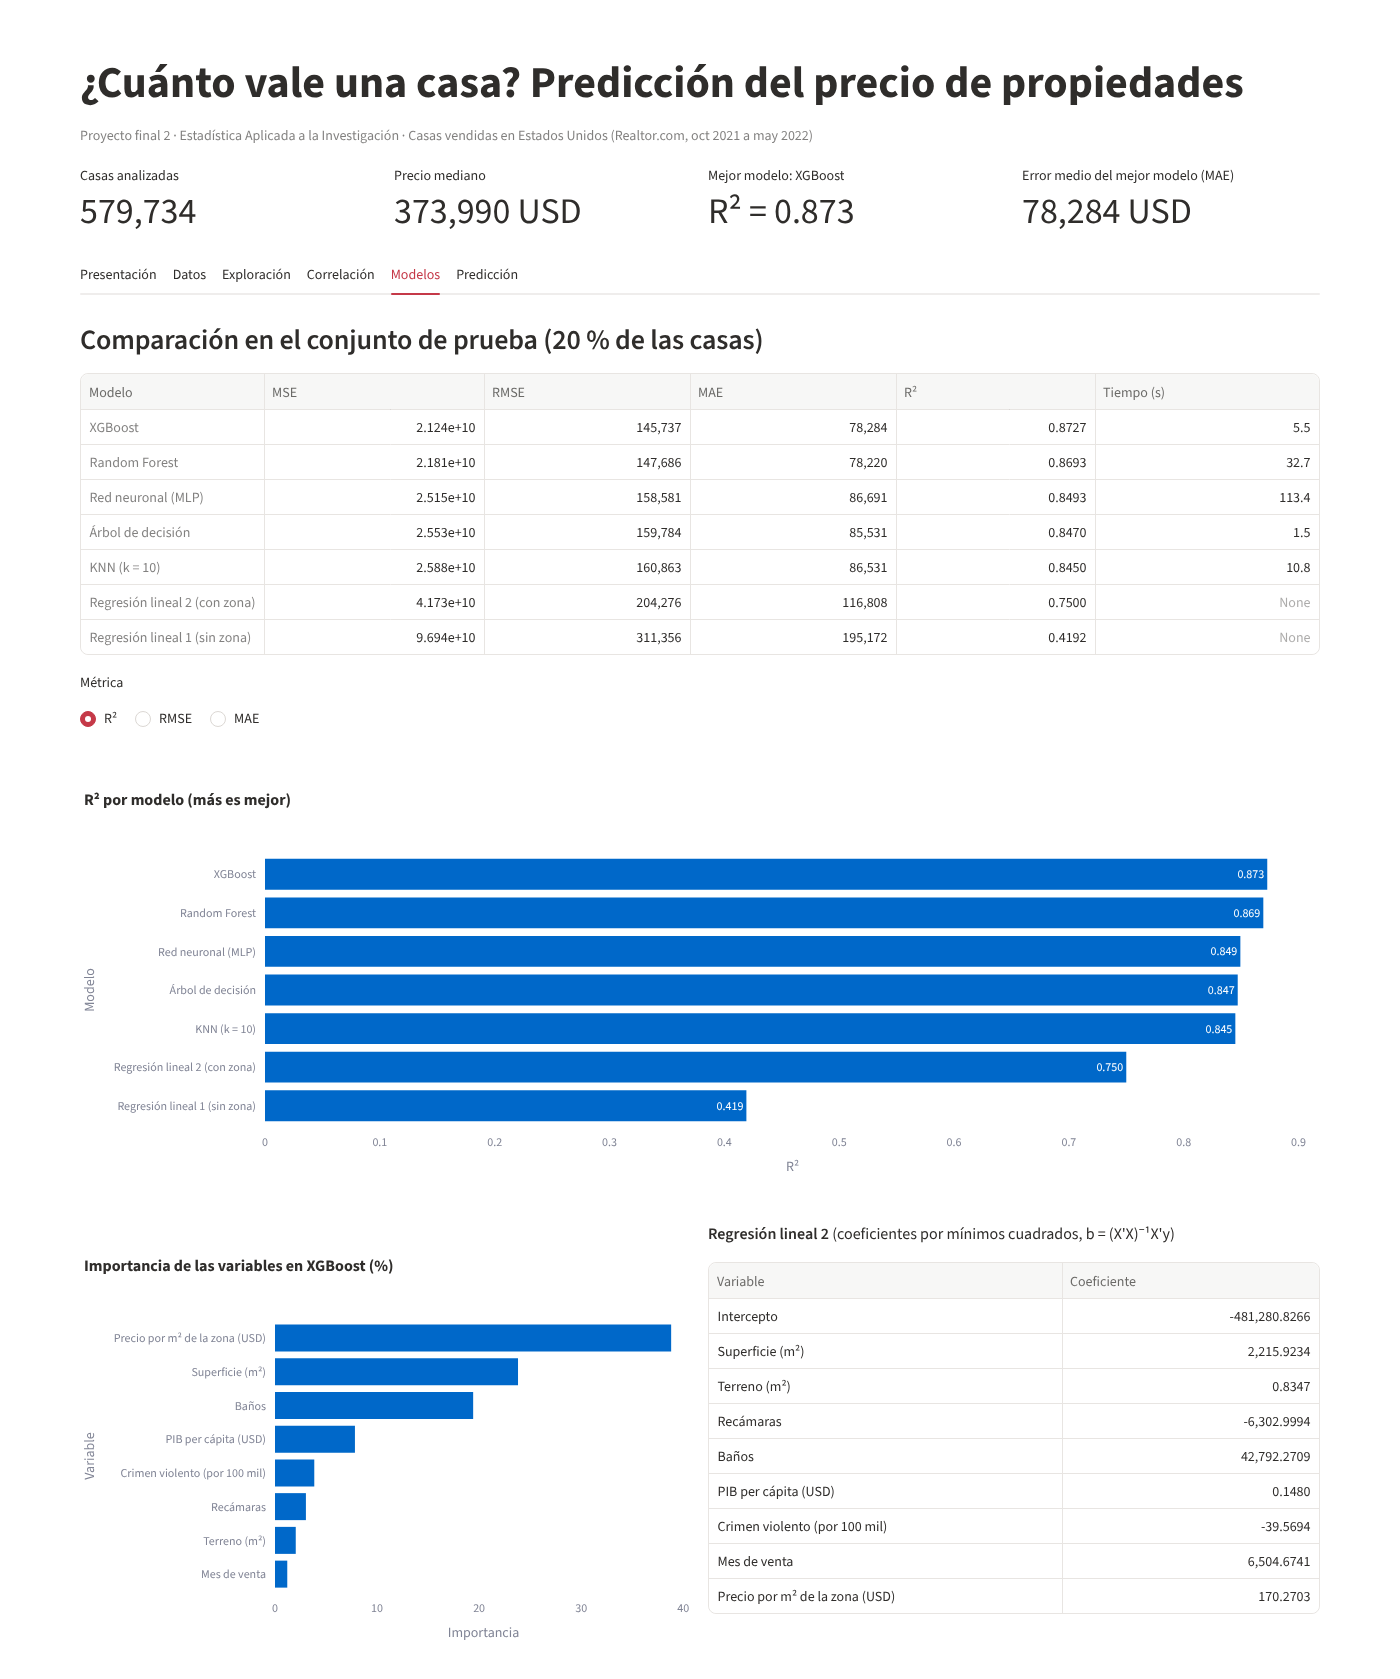
\includegraphics[width=\textwidth]{figuras/dashboard_modelos.png}
\caption{Dashboard: comparación de modelos.}
\end{figure}

\begin{figure}[H]
\centering
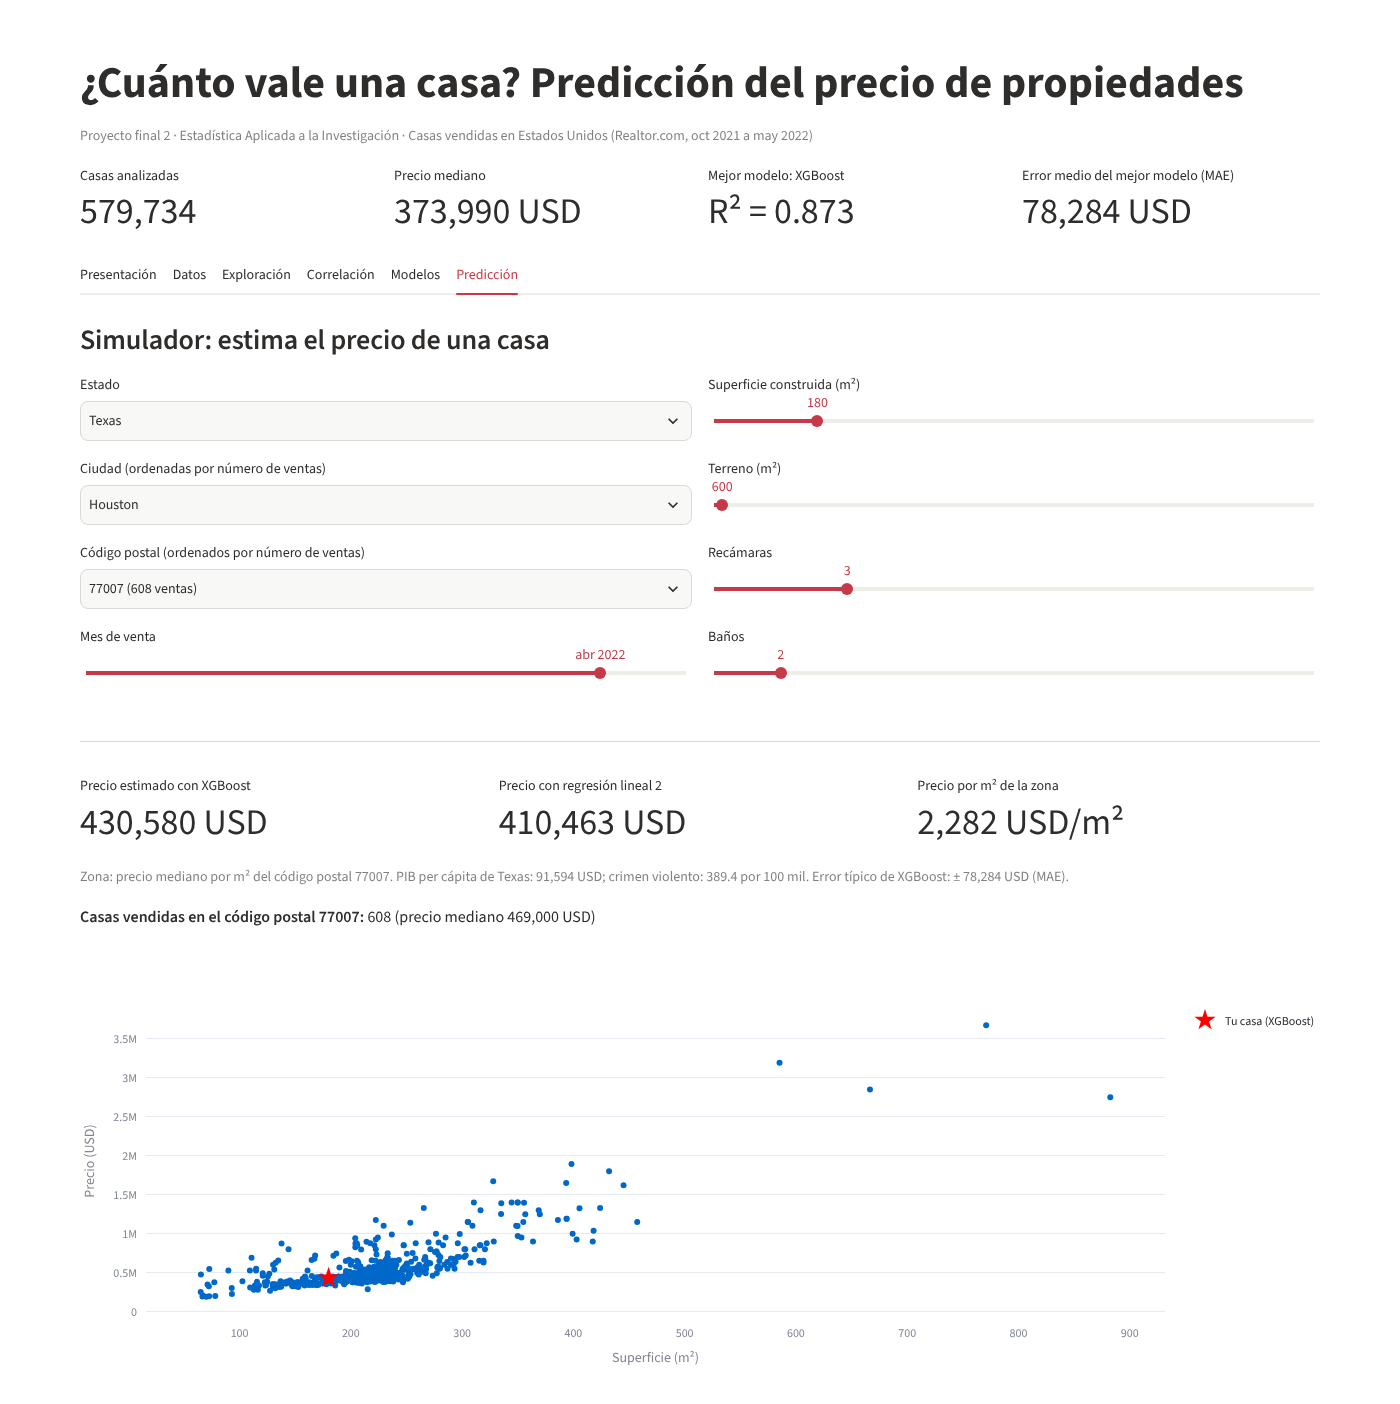
\includegraphics[width=\textwidth]{figuras/dashboard_prediccion.png}
\caption{Dashboard: simulador de precio.}
\end{figure}

%%%%%%%%%%%%%%%%%%%%%%%%%%%%%%%%%%%%%%%%%%%%%%%%%%%%%%%%%%%%%%%%%%%%%%%%%%%
\section*{Referencias}
\addcontentsline{toc}{section}{Referencias}
\begin{itemize}[leftmargin=*,label={}]
  \item Bureau of Economic Analysis. (2026). \emph{Gross domestic product by state and personal income by state}. U.S. Department of Commerce. \url{https://www.bea.gov}
  \item Federal Bureau of Investigation. (2025). \emph{Crime Data Explorer: Uniform Crime Reporting Program}. U.S. Department of Justice. \url{https://cde.ucr.cjis.gov}
  \item Sakib, A. S. (2024). \emph{USA real estate dataset} [Conjunto de datos]. Kaggle. \url{https://www.kaggle.com/datasets/ahmedshahriarsakib/usa-real-estate-dataset}
  \item Wikipedia. (2026). \emph{List of U.S. states and territories by GDP}. Recuperado el 23 de noviembre de 2026 de \url{https://en.wikipedia.org/wiki/List_of_U.S._states_and_territories_by_GDP}
  \item Wikipedia. (2026). \emph{List of U.S. states and territories by violent crime rate}. Recuperado el 23 de noviembre de 2026 de \url{https://en.wikipedia.org/wiki/List_of_U.S._states_and_territories_by_violent_crime_rate}
\end{itemize}

%%%%%%%%%%%%%%%%%%%%%%%%%%%%%%%%%%%%%%%%%%%%%%%%%%%%%%%%%%%%%%%%%%%%%%%%%%%
\clearpage
\appendix
\section{Cálculos desarrollados}\label{sec:anexo}

\subsection{Regresión del modelo 1 por matrices}

Con $n = 463,787$ casas de entrenamiento y $k = 7$ variables, la matriz $\mathbf{X}$ tiene 463,787 filas y 8 columnas: una de unos y las 7 variables. Cada elemento de $\mathbf{X}'\mathbf{X}$ es una suma de productos; por ejemplo, el de la fila 1 y columna 1 es $n$, el de la fila 1 y columna 2 es $\sum x_{\text{Sup}}$ y el de la fila 2 y columna 2 es $\sum x_{\text{Sup}}^2$. La notación $a\,\mathrm{E}k$ significa $a \times 10^k$.

\begin{table}[H]
\centering
\caption{Matriz $\mathbf{X}'\mathbf{X}$ ($8 \times 8$).}
\scriptsize\setlength{\tabcolsep}{2.5pt}
\begin{tabular}{l*{8}{r}}
\toprule
 & 1 & Sup. & Terr. & Rec. & Baños & PIB & Crimen & Mes \\
\midrule
\textbf{1} & $4.638{\scriptstyle\,\mathrm{E}5}$ & $8.384{\scriptstyle\,\mathrm{E}7}$ & $9.645{\scriptstyle\,\mathrm{E}8}$ & $1.526{\scriptstyle\,\mathrm{E}6}$ & $1.129{\scriptstyle\,\mathrm{E}6}$ & $4.242{\scriptstyle\,\mathrm{E}10}$ & $1.699{\scriptstyle\,\mathrm{E}8}$ & $1.748{\scriptstyle\,\mathrm{E}6}$ \\
\textbf{Sup.} & $8.384{\scriptstyle\,\mathrm{E}7}$ & $1.851{\scriptstyle\,\mathrm{E}10}$ & $1.943{\scriptstyle\,\mathrm{E}11}$ & $3.002{\scriptstyle\,\mathrm{E}8}$ & $2.338{\scriptstyle\,\mathrm{E}8}$ & $7.674{\scriptstyle\,\mathrm{E}12}$ & $3.060{\scriptstyle\,\mathrm{E}10}$ & $3.169{\scriptstyle\,\mathrm{E}8}$ \\
\textbf{Terr.} & $9.645{\scriptstyle\,\mathrm{E}8}$ & $1.943{\scriptstyle\,\mathrm{E}11}$ & $1.106{\scriptstyle\,\mathrm{E}13}$ & $3.165{\scriptstyle\,\mathrm{E}9}$ & $2.447{\scriptstyle\,\mathrm{E}9}$ & $8.735{\scriptstyle\,\mathrm{E}13}$ & $3.475{\scriptstyle\,\mathrm{E}11}$ & $3.572{\scriptstyle\,\mathrm{E}9}$ \\
\textbf{Rec.} & $1.526{\scriptstyle\,\mathrm{E}6}$ & $3.002{\scriptstyle\,\mathrm{E}8}$ & $3.165{\scriptstyle\,\mathrm{E}9}$ & $5.441{\scriptstyle\,\mathrm{E}6}$ & $3.964{\scriptstyle\,\mathrm{E}6}$ & $1.399{\scriptstyle\,\mathrm{E}11}$ & $5.580{\scriptstyle\,\mathrm{E}8}$ & $5.743{\scriptstyle\,\mathrm{E}6}$ \\
\textbf{Baños} & $1.129{\scriptstyle\,\mathrm{E}6}$ & $2.338{\scriptstyle\,\mathrm{E}8}$ & $2.447{\scriptstyle\,\mathrm{E}9}$ & $3.964{\scriptstyle\,\mathrm{E}6}$ & $3.195{\scriptstyle\,\mathrm{E}6}$ & $1.035{\scriptstyle\,\mathrm{E}11}$ & $4.144{\scriptstyle\,\mathrm{E}8}$ & $4.268{\scriptstyle\,\mathrm{E}6}$ \\
\textbf{PIB} & $4.242{\scriptstyle\,\mathrm{E}10}$ & $7.674{\scriptstyle\,\mathrm{E}12}$ & $8.735{\scriptstyle\,\mathrm{E}13}$ & $1.399{\scriptstyle\,\mathrm{E}11}$ & $1.035{\scriptstyle\,\mathrm{E}11}$ & $4.029{\scriptstyle\,\mathrm{E}15}$ & $1.585{\scriptstyle\,\mathrm{E}13}$ & $1.595{\scriptstyle\,\mathrm{E}11}$ \\
\textbf{Crimen} & $1.699{\scriptstyle\,\mathrm{E}8}$ & $3.060{\scriptstyle\,\mathrm{E}10}$ & $3.475{\scriptstyle\,\mathrm{E}11}$ & $5.580{\scriptstyle\,\mathrm{E}8}$ & $4.144{\scriptstyle\,\mathrm{E}8}$ & $1.585{\scriptstyle\,\mathrm{E}13}$ & $6.724{\scriptstyle\,\mathrm{E}10}$ & $6.452{\scriptstyle\,\mathrm{E}8}$ \\
\textbf{Mes} & $1.748{\scriptstyle\,\mathrm{E}6}$ & $3.169{\scriptstyle\,\mathrm{E}8}$ & $3.572{\scriptstyle\,\mathrm{E}9}$ & $5.743{\scriptstyle\,\mathrm{E}6}$ & $4.268{\scriptstyle\,\mathrm{E}6}$ & $1.595{\scriptstyle\,\mathrm{E}11}$ & $6.452{\scriptstyle\,\mathrm{E}8}$ & $8.167{\scriptstyle\,\mathrm{E}6}$ \\
\bottomrule
\end{tabular}
\end{table}

La inversa se obtuvo como $\paren{\mathbf{X}'\mathbf{X}}^{-1} = \dfrac{1}{\det\paren{\mathbf{X}'\mathbf{X}}}\,\operatorname{adj}\paren{\mathbf{X}'\mathbf{X}}$, calculada con NumPy (para una matriz de $8 \times 8$ el cálculo de cofactores a mano no es práctico).

\begin{table}[H]
\centering
\caption{Matriz inversa $\paren{\mathbf{X}'\mathbf{X}}^{-1}$.}
\scriptsize\setlength{\tabcolsep}{2.5pt}
\begin{tabular}{l*{8}{r}}
\toprule
 & 1 & Sup. & Terr. & Rec. & Baños & PIB & Crimen & Mes \\
\midrule
\textbf{1} & $9.982{\scriptstyle\,\mathrm{E}-5}$ & $2.130{\scriptstyle\,\mathrm{E}-8}$ & $-3.511{\scriptstyle\,\mathrm{E}-10}$ & $-7.415{\scriptstyle\,\mathrm{E}-6}$ & $-2.185{\scriptstyle\,\mathrm{E}-6}$ & $-5.162{\scriptstyle\,\mathrm{E}-10}$ & $-4.031{\scriptstyle\,\mathrm{E}-8}$ & $-2.410{\scriptstyle\,\mathrm{E}-6}$ \\
\textbf{Sup.} & $2.130{\scriptstyle\,\mathrm{E}-8}$ & $8.745{\scriptstyle\,\mathrm{E}-10}$ & $-1.446{\scriptstyle\,\mathrm{E}-12}$ & $-2.427{\scriptstyle\,\mathrm{E}-8}$ & $-4.416{\scriptstyle\,\mathrm{E}-8}$ & $5.903{\scriptstyle\,\mathrm{E}-14}$ & $1.831{\scriptstyle\,\mathrm{E}-11}$ & $-3.069{\scriptstyle\,\mathrm{E}-10}$ \\
\textbf{Terr.} & $-3.511{\scriptstyle\,\mathrm{E}-10}$ & $-1.446{\scriptstyle\,\mathrm{E}-12}$ & $1.134{\scriptstyle\,\mathrm{E}-13}$ & $6.563{\scriptstyle\,\mathrm{E}-11}$ & $3.353{\scriptstyle\,\mathrm{E}-11}$ & $3.315{\scriptstyle\,\mathrm{E}-16}$ & $8.105{\scriptstyle\,\mathrm{E}-14}$ & $5.095{\scriptstyle\,\mathrm{E}-12}$ \\
\textbf{Rec.} & $-7.415{\scriptstyle\,\mathrm{E}-6}$ & $-2.427{\scriptstyle\,\mathrm{E}-8}$ & $6.563{\scriptstyle\,\mathrm{E}-11}$ & $4.239{\scriptstyle\,\mathrm{E}-6}$ & $-7.762{\scriptstyle\,\mathrm{E}-7}$ & $-9.834{\scriptstyle\,\mathrm{E}-12}$ & $1.038{\scriptstyle\,\mathrm{E}-9}$ & $3.484{\scriptstyle\,\mathrm{E}-8}$ \\
\textbf{Baños} & $-2.185{\scriptstyle\,\mathrm{E}-6}$ & $-4.416{\scriptstyle\,\mathrm{E}-8}$ & $3.353{\scriptstyle\,\mathrm{E}-11}$ & $-7.762{\scriptstyle\,\mathrm{E}-7}$ & $5.598{\scriptstyle\,\mathrm{E}-6}$ & $-2.285{\scriptstyle\,\mathrm{E}-12}$ & $-1.872{\scriptstyle\,\mathrm{E}-9}$ & $-2.122{\scriptstyle\,\mathrm{E}-8}$ \\
\textbf{PIB} & $-5.162{\scriptstyle\,\mathrm{E}-10}$ & $5.903{\scriptstyle\,\mathrm{E}-14}$ & $3.315{\scriptstyle\,\mathrm{E}-16}$ & $-9.834{\scriptstyle\,\mathrm{E}-12}$ & $-2.285{\scriptstyle\,\mathrm{E}-12}$ & $7.752{\scriptstyle\,\mathrm{E}-15}$ & $-4.866{\scriptstyle\,\mathrm{E}-13}$ & $3.187{\scriptstyle\,\mathrm{E}-12}$ \\
\textbf{Crimen} & $-4.031{\scriptstyle\,\mathrm{E}-8}$ & $1.831{\scriptstyle\,\mathrm{E}-11}$ & $8.105{\scriptstyle\,\mathrm{E}-14}$ & $1.038{\scriptstyle\,\mathrm{E}-9}$ & $-1.872{\scriptstyle\,\mathrm{E}-9}$ & $-4.866{\scriptstyle\,\mathrm{E}-13}$ & $2.334{\scriptstyle\,\mathrm{E}-10}$ & $-8.098{\scriptstyle\,\mathrm{E}-10}$ \\
\textbf{Mes} & $-2.410{\scriptstyle\,\mathrm{E}-6}$ & $-3.069{\scriptstyle\,\mathrm{E}-10}$ & $5.095{\scriptstyle\,\mathrm{E}-12}$ & $3.484{\scriptstyle\,\mathrm{E}-8}$ & $-2.122{\scriptstyle\,\mathrm{E}-8}$ & $3.187{\scriptstyle\,\mathrm{E}-12}$ & $-8.098{\scriptstyle\,\mathrm{E}-10}$ & $6.363{\scriptstyle\,\mathrm{E}-7}$ \\
\bottomrule
\end{tabular}
\end{table}

\begin{table}[H]
\centering
\caption{Vector $\mathbf{X}'\mathbf{y}$ y coeficientes $\mathbf{b} = \paren{\mathbf{X}'\mathbf{X}}^{-1}\mathbf{X}'\mathbf{y}$.}
\small
\begin{tabular}{lrr}
\toprule
Variable & $\mathbf{X}'\mathbf{y}$ & $\mathbf{b}$ \\
\midrule
Intercepto & $2.2281\times10^{11}$ & -778110.2159 \\
Superficie (m$^2$) & $4.8883\times10^{13}$ & 1991.3590 \\
Terreno (m$^2$) & $4.9401\times10^{14}$ & -1.0298 \\
Recámaras & $7.9311\times10^{11}$ & -29908.5427 \\
Baños & $6.3653\times10^{11}$ & 90715.5957 \\
PIB per cápita (USD) & $2.1437\times10^{16}$ & 5.9369 \\
Crimen violento (por 100 mil) & $8.5859\times10^{13}$ & 494.3477 \\
Mes de venta & $8.6596\times10^{11}$ & 14351.3502 \\
\bottomrule
\end{tabular}
\end{table}

Por ejemplo, $b_0$ es el producto de la primera fila de la inversa por el vector $\mathbf{X}'\mathbf{y}$:
$$ b_0 = \sum_{j=1}^{8} \paren{\mathbf{X}'\mathbf{X}}^{-1}_{1j}\,\paren{\mathbf{X}'\mathbf{y}}_j = -778110.2159 $$

Ecuación del modelo 1:
$$ \hat{y} = -778,110.22 + 1,991.36\,\text{Sup} - 1.0298\,\text{Terr} - 29,908.54\,\text{Rec} $$
$$ \quad + 90,715.60\,\text{Baños} + 5.9369\,\text{PIB} + 494.35\,\text{Crimen} + 14,351.35\,\text{Mes} $$

\subsection{Prueba de significancia de la correlación}

Para la superficie, con $r = 0.5323$ y $n = 579,734$:
$$ t = \frac{r\sqrt{n-2}}{\sqrt{1-r^2}} = \frac{0.5323\sqrt{579{,}732}}{\sqrt{1-0.5323^2}} = \frac{0.5323 \times 761.40}{0.8466} = 478.73 $$
El valor crítico con $\alpha = 0.05$ y $gl = 579{,}732$ es $t_{0.025} \approx 1.96$. Como $478.73 > 1.96$, se rechaza $H_0$: la correlación entre la superficie y el precio es significativa.

\subsection{Métricas del mejor modelo (XGBoost)}

Con $n = 115{,}947$ casas de prueba:
$$ MSE = \frac{\sum \paren{y_i - \hat{y}_i}^2}{n} = 2.1239\times10^{10}\ \text{USD}^2 $$
$$ RMSE = \sqrt{MSE} = \sqrt{2.1239\times10^{10}} = 145{,}737\ \text{USD} $$
$$ MAE = \frac{\sum \left|y_i - \hat{y}_i\right|}{n} = 78{,}284\ \text{USD} $$
$$ R^2 = 1 - \frac{SC_{error}}{SC_{total}} = 0.8727 $$
Es decir, XGBoost explica el 87.3\,\% de la variación del precio de las casas que no vio al entrenar.

\end{document}
